%!TEX root = ../thesis.tex
% NIR-information

\chapter{Information content in the \nir{}}
\label{cha:nir_content}

The work presented in this chapter focuses on calculating and analysing the information content of stellar spectra, specifically the radial velocity precision of M-dwarf spectra in the \nir{}.
This work is not directly related to detecting exoplanet atmospheres themselves but will aid in future exoplanet discoveries.
For instance, the fundamental radial velocity precision of {M-dwarf} spectra attainable at different wavelength regions calculated in~\citet{figueira_radial_2016} was used to influence some design choices of two \nir{} spectrographs, {SPIRou} and {NIRPS}.
Understanding the underlying precision of different spectral types can also allow {RV} surveys to adjust the focus the target selection, or optimize the exposure time of different spectral types.
This can help in detecting the presence of ``habitable Earth-like'' planets around {M-dwarfs} which have become a prime target with the recent \nir{} spectrographs.

The purpose of the work presented in this chapter is to extend the work of~\citet{figueira_radial_2016}, computing the theoretical {RV} precision of synthetic stellar spectra over a wider range of situations.
A investigation into the effect of \Logg{} and \feh{} on precision is performed and a preliminary comparison of {RV} precision of the recently observed \nir{} {M-dwarf} spectra from {CARMENES} library and their synthetic counterparts is given.
This is to test how the {RV} precision of synthetic models compares to reality.
Computations of the {RV} precision of synthetic spectral libraries are given, which were provided for exposure time calculators of {NIRPS} and {SPIRou}. 


\section{Overview}
\label{sec:precision_overview}
The pursuit of detecting exoplanets, especially ``habitable'' and ``Earth-like'' planets, requires state-of-the-art instrumentation with high precision.
Several new high-resolution \nir{} spectrographs are becoming available now and in the near future, not limited to {CARMENES}, {NIRPS}, {SPIRou} and {CRIRES+} (see \cref{subsec:new_generation}).
One science objective common to all four instruments is the detection of small mass planets around {M-dwarf} stars utilizing the radial velocity technique.
As the {RV} amplitude is \(\kone\propto {P}^{-{1/2}}{\mone}^{-2/3}\) (\cref{eqn:k_relation}), the induced {RV} wobble from a similarly sized exoplanet is larger around an M-dwarf star, making the {RV} signal from lower mass exoplanets easier to detect.
Also the cooler M-dwarfs have habitable zones closer to the star, at shorter orbital periods that again have a stronger {RV} amplitude.
Making it easier to detect small mass planets in the habitable zone of {M-Dwarfs}.

To calculate and predict the information content attainable from {M-dwarfs} in the \nir{}~\cite{figueira_radial_2016} utilized the {PHOENIX-ACES} library of synthetic spectra.
This helped to aid the direction of instrument design by identifying the wavelength regions with the best {RV} precision, but can also help in the planning of observations, by understanding how the precision changes with spectral type and observed {\snr{}}.
However, the synthetic spectra do not quite match reality and a comparison between theoretical and observed is needed.
\citet{artigau_optical_2018} recently compared optical (HARPS, {ESpaDOnS) and \nir{} (CRIRES) archival spectra of the M-dwarf, Barnard's Star, to synthetic spectra.
They found that state-of-the-art atmosphere models over-predict the {RV} content \emph{Y}- and \emph{J}-band {RV} by more than a factor of \(\sim\)2, while under-predicting the \emph{H}- and \emph{K}-band content by half.
A similar comparison will be made in this work to {CARMENES} spectra.

Recent results regarding the measured performance of the CARMENES survey~\citep{reiners_carmenes_2018,quirrenbach_carmenes_2018} find that the {RV} in the \nir{} is worse than the pre-survey predictions.
Precisions of 1--2\mps{} have been achieved in the optical but only 5--10\mps{} in the \nir{}.
However, comparing RV precision in different wavelength bands~\citet{quirrenbach_carmenes_2018} find a ``sweet spot'' around 0.7--0.8\um{} with deep \ce{TiO} bands providing rich {RV} information in mid-M dwarfs.


%!TEX root = ../../thesis.tex


\subsection{Fundamental photon noise limitation}
\label{subsec:fundamental_precision}
A technique to calculate the theoretical radial velocity precision of a spectrum using the full spectral information in an optimal way was first presented by~\citet{connes_absolute_1985}.
Here the radial velocity precision derivation following~\citet{connes_absolute_1985, bouchy_fundamental_2001, figueira_radial_2016} is provided.

\begin{figure}
    \centering
    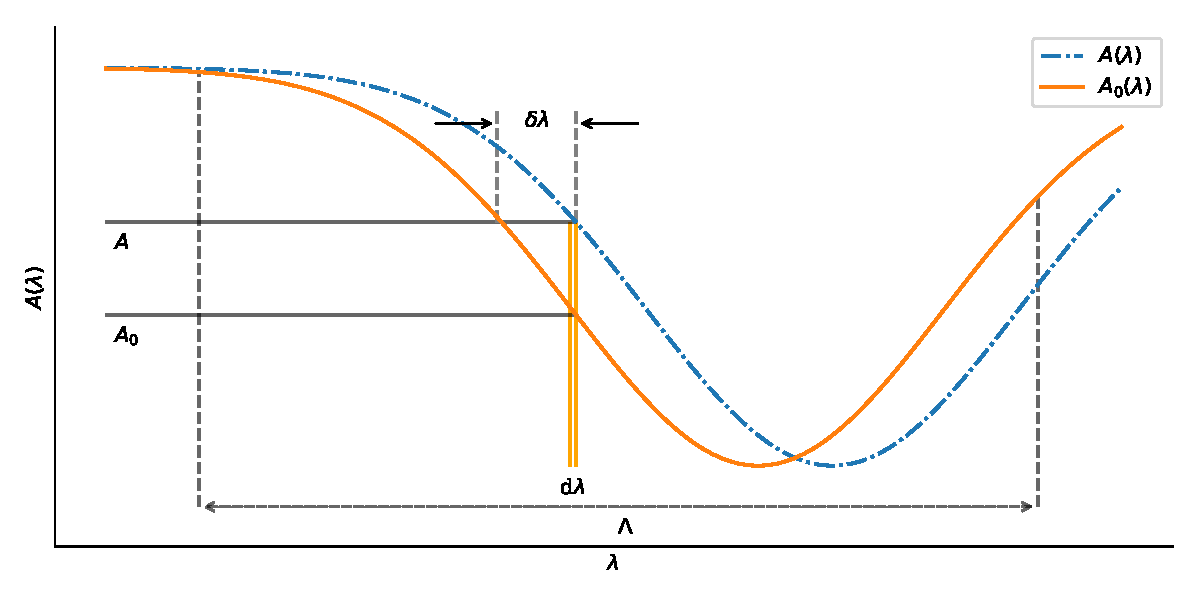
\includegraphics[width=0.8\linewidth]{figures/information-content/precision_plot.pdf}
    \caption[Demonstration of a shifted arbitrary spectral line.]{Arbitrary spectral line with a shift \(\delta \lambda\), inspired by~\citet{connes_absolute_1985}.
        \(\Lambda\) is the wavelength range considered.}
    \label{fig:precisionderivation}
\end{figure}
\todo{add \(\delta A\) to plots}

For demonstration purposes \cref{fig:precisionderivation} shows a portion of an arbitrary spectrum \(A(\lambda)\), for demonstration purposes over a wavelength range \(\Lambda\).
Here \({A}_{0}(\lambda)\) is the reference spectrum while \(A(\lambda)\) is observed some later time with an apparent wavelength shift observed.
The majority of a single Gaussian line is shown as spectral lines contain the most information but the presence of spectral lines is not a requirement for the derivation.

The Doppler shift of a spectrum is given by:
\begin{equation}
\frac{\delta V}{c} = \frac{\delta \lambda}{\lambda},
\label{eqn:dopplershift}
\end{equation}
where \(c\) is the speed of light in a vacuum, and \(\delta \lambda\) is the shift in wavelength \(\lambda\) due to the velocity \(\delta V\).

\todo{intensity change from connes is vertically in the slice d lambda}

Using basic calculus \(\delta y = \pd{y}{x} \delta x \nonumber\), and for a Doppler shift that is small compared to the line-width\footnote{Although~\citet{connes_absolute_1985} show that the approximation in \cref{eqn:intensitychange} is adequate under all circumstances.}, the observable intensity change in a wavelength slice \(d \lambda\) (or at a given pixel) can be expressed by:
\begin{equation}
\delta A(i) = A(i) - {A}_{0}(i) \simeq \pd{{A}_{0}(i)}{\lambda(i)} \delta \lambda = \pd{{A}_{0}(i)}{\lambda(i)} \frac{\delta V(i)}{c}\lambda(i).
\label{eqn:intensitychange}
\end{equation}

Rearranging \cref{eqn:intensitychange} for \(\delta \lambda\) and combining it with \cref{eqn:dopplershift}, the Doppler shift then becomes:
\begin{equation}
\frac{\delta V(i)}{c} = \frac{A(i) - {A}_{0}(i) }{\lambda(i) (\partial {A}_{0}(i)/\partial \lambda(i))} \label{eqn:delta_v_i}
\end{equation}

This equation shows that the radial velocity measured at pixel {\(i\)}, through a change in the intensity in the recorded spectrum, \(A(i)-{A}_{0}(i)\), and inversely proportional to the slope of the spectrum, \({\partial {A}_{0}(i)}/{\partial \lambda(i)}\).
\Cref{eqn:delta_v_i} provides a separate measurement of the radial velocity shift for every pixel, \(i\), in the spectrum.
The sensitivity of the velocity measurement can be improved, and the noise decreased by using the information from the whole spectral range, \(\Lambda\).
This is achieved by taking the weighted average\footnote{Weighted average on x is \(\bar{x} = \frac{\sum{ x(i)W(i)}}{\sum {W(i)}}\)} over all pixels in the spectral range using an optimal pixel weight \(W(i)\).

\begin{equation}
\overline{\frac{\delta V}{c}} = \frac{\sum{\frac{\delta V(i)}{c}W(i)}}{\sum {W(i)}}.
\end{equation}

Statistically, the optimal weights are proportional to the inverse square of the individual dispersion (variance),
\begin{equation}
W(i) = \frac{1}{{\left(\frac{\delta V_{\rms}(i)}{c}\right)}^{2}}, \label{eqn:weights}
\end{equation}
where \(X_{\rms}\) is the dispersion on the quantity \(X\).

The individual dispersion of the velocity measurement \(\delta V_{\rms}(i)\) is the dispersion that would result from several measurements of the reference spectrum all with the same Doppler shift (e.g.\ zero).
\Cref{eqn:delta_v_i} thus becomes:
\begin{equation}
\frac{\delta V_{\rms}(i)}{c} = \frac{{[A(i) - {A}_{0}(i)]}_{\rms} }{\lambda(i) (\partial {A}_{0}(i)/\partial \lambda(i))}.
\label{eqn:delta_v_i_rms}
\end{equation}
The noise of the spectrum \(A\) is the quadratic sum of the photon noise \(\sqrt{A}\) and the detector noise \({\sigma}_{D}\).
The spectrum \({A}_{0}\) is considered noise free.

\begin{equation}
{[{A(i)-{A}_{0}(i)}]}_{\rms} = {[{A(i)} - 0]}_{\rms} = \sqrt{{\sqrt{A(i)}}^{2} + {{\sigma}^{2}}_{D}} \label{eqn:noise}
\end{equation}

Considering that the Doppler shift is small and that \(A\) and \({A}_{0}\) have the same intensity level, then \(A = {A}_{0}\) can be set.
Using \cref{eqn:delta_v_i,eqn:weights,eqn:noise} the optimum weights then become solely dependent on the reference spectrum.

\begin{equation}
W(i) = \frac{{\lambda}^{2}(i) {({\partial {A}_{0}(i)}/{\partial \lambda(i)})}^{2}}{A_0(i) + {\sigma}^{2}_{D}} \label{eqn:optimal_weight}
\end{equation}

This weighting function can be modified to mask out and eliminate unwanted lines in the spectrum (see \cref{subsec:masking_function}).
For instance setting the particular pixel weights to zero to remove any telluric absorption lines in the observed spectra.

With the optimal weights set, the weighed average velocity change measured from the full spectral range \(\Lambda\), is given by:

\begin{align}
\frac{\overline{\delta V}}{c} &= \frac{
    \sum{
        \frac
        {A(i) - {A}_{0}(i)}{
            \lambda(i) \left({\partial {A}_{0}(i)}/{\partial \lambda(i)}\right)} W(i)}
}
{\sum{{W(i)}}} \\
&= \frac{
    \sum {
        \frac
        {A(i) - {A}_{0}(i)}
        {\lambda(i) (\partial {A}_{0}(i)/\partial \lambda(i))}
        \frac
        {{\lambda}^{2}(i) {({\partial {A}_{0}(i)}/{\partial \lambda(i)})}^{2}}
        {A_{0}(i) + {\sigma}^{2}_{D}}
    }
}
{\sum{{W(i)}}} \\
&= \frac{
    \sum { 
        (A(i) - {A}_{0}(i))
        \frac
        {\lambda(i) {\partial {A}_{0}(i)}/{\partial \lambda(i)}}
        {A_{0}(i) + {\sigma}^{2}_{D}}
    }
}
{\sum{{W(i)}}} \\
&= \frac{\sum{(A(i) - {A}_{0}(i)){\left(\frac{W(i)}{{A}_{0}(i) +{\sigma}_{D}^{2}}\right)}^{1/2}}}{\sum{W(i)}}
\label{eqn:delta_v_eqarray}
\end{align}

The important quantity for {RV} measurements is not just the velocity values themselves but also the dispersion (or uncertainty) on the measured velocity, the {RV} precision \(\delta V_{\rms}\), from the spectrum.
This allows one to assess the planetary detectability limitations attainable in the spectra.
From rearranging \cref{eqn:weights} the dispersion is given by:
\begin{equation}
\overline{\frac{\delta V_{\rms}}{c}} = \frac{1}{\sqrt{\sum{\,W(i)}}} = \frac{1}{Q \sqrt{\sum{\,{A}_{0}(i)}}}.\label{eqn:dv_rms}
\end{equation}
With \cref{eqn:dv_rms} the velocity precision is inversely proportional to the sum of the optimal pixel weights.
Here \(Q\) is a spectral quality factor, defined for the pure photon noise case in~\cite{connes_absolute_1985, connes_demonstration_1996}, as:
\begin{equation}
Q \equiv \frac{\sqrt{\sum{\,W(i)}}}{\sqrt{\sum{\,{A}_{0}(i)}}} = \frac{\sqrt{\sum{\,\frac{{\lambda}^{2}(i) {({\partial {A}_{0}(i)}/{\partial \lambda(i)})}^{2}}{A_0(i) + {\sigma}^{2}_{D}}}}}{\sqrt{\sum{\,{A}_{0}(i)}}}.
\end{equation}

The pure photon noise case is exclusively considered here in a high signal-to-noise regime in which \({A(i) + \sigma_{D}^{2}} \sim {A(i)}\) can be approximated.
The quality factor, \(Q\), becomes flux independent and is purely a function of the spectral profile within the spectral range considered\footnote{In the case of pure detector noise case the fluctuations in \(A\) are independent of the spectrum \(A\) and the quality factor is \({Q}_{D} = \frac{\sqrt{\sum{{\lambda}^{2} {(\partial {A}_{0}(i)/\partial \lambda(i))}^{2}}}}{\sum{\, {A}_{0}(i)}}\) as derived by~\cite{connes_absolute_1985}.}.
It is a measure of the line richness i.e.\ that quantity and depth of the lines.
For example a spectrum with many sharp lines will have a high \(Q\).
The instrumental resolution of the spectrograph also effects the spectral quality as it induces line broadening.

The radial velocity precision or uncertainty can be rearranged in terms of the spectral quality;
\begin{equation}
\delta V_{\rms} = \frac{c}{Q \sqrt{\sum {\,{A}_{0}(i)}}} = \frac{c}{Q \sqrt{{N}_{{e}^{-}}}} \approx \frac{c}{Q \cdot \snr{}},  \label{eqn:snr_relation}
\end{equation}
where \(\sum {A}_{0}(i) = {N}_{{e}^{-}}\) is considered to be the total number of photo-electrons \({N}_{{e}^{-}}\) counted in the spectral range considered, and \(\snr{}=\sqrt{N_{{e}^{-}}}\) for large \(N_{{e}^{-}}\).

The number of photo-electrons counted \(N_{{e}^{-}}\) in an observed spectrum depends on many factors, such as: the stellar magnitude, detector efficiency and integration time.
It can be estimated using
\begin{equation}
N_{{e}^{-}} = P_{avg} * S_{tel} * \texp * \alpha* \Lambda, \label{eqn:Ne}
\end{equation}
where \(P_{avg}\) is the average monochromatic stellar brightness
across the wavelength range \(\Lambda\) in \si{\photons\per\second\per\centi\metre\squared\per\centi\metre},
\(S_{tel}\) is the telescope collecting area in \si{\centi\metre\squared},
\(\texp\) is the integration time in \si{\second}, and \(\alpha\) the is overall system efficiency (including atmosphere, telescope, spectrograph and detector).

This technique has been tested and demonstrated on observations by~\citet{connes_demonstration_1996} and been used to predict the accuracy or performance limits of new spectrograph instrumentation~\citep[e.g.][]{connes_absolute_1985,butler_attaining_1996,bouchy_fundamental_2001} and has influence the design (and use) of spectrographs, e.g.\ {SPIRou}~\citep{artigau_spirou_2014,figueira_radial_2016}.
However,~\citet{figueira_radial_2016} bypass the calculation of \(N_{{e}^{-}}\) in \cref{eqn:Ne} by scaling the synthetic spectral models to a specific \snr{} level instead.

In the case of several \(\delta V\) measurements computed for \(k\) spectral slices (or spectral orders) then the error on the average \(\overline{\delta V}\) is given by the error on a weighted average:
\begin{equation}
\overline{\delta {V}_{\rms}} = \frac{1}{\sqrt{\sum_k{{(\frac{1}{\delta V_{\rms}(k)})}^{2}}}}. \label{eqn:weighted_average_error}
\end{equation}

A separate general formula for {RV} precision, discussed in \cref{section:rv_precision}, is given by~\citet{hatzes_spectrograph_1992} in terms of general spectral parameters:
\begin{equation}
\delta V_{\rms} = \frac{1}{\sqrt{F} \sqrt{\Lambda} {R}^{1.5}}
\end{equation}
where $\sqrt{F}$ represents the \snr{} of the spectrum in the {Poisson}-noise dominated regime, and \(R\) is the spectral resolution.
The $\Lambda$ comes from assuming a homogeneous distribution of lines, with the same line properties, per unit length.




\section{Deriving RV for synthetic spectra}

\subsection{Prepare {PHOENIX} aces models}:
\# see~\citet{figueira_radial_2016}

Convert SED to counts.


Scale to 100 \snr{} per resolution element in \emph{J}-band.

Convolutions

\subsection{Rotational convolution}
\label{subsec:rotational_convolution}
Stellar rotation has the affect of broadening spectral lines as the different portions of the stellar surface have a variation of radial velocity between \(\pm v \sin i\).
Rotation is applied to a non-rotating spectrum by convolution with a rotation kernel.
The stellar rotational kernel used is given by~\citet{gray_observation_2005};

\todo{top view diagram of rotation?}

\begin{align}
G(\Delta\lambda) &= \frac{2(1-\epsilon){[1-{(\Delta\lambda /{\Delta\lambda}_{L})}^{2}]}^{1/2} +   \frac{1}{2}\pi\epsilon[1-{(\Delta\lambda /{\Delta\lambda}_{L})}^{2}]}{\pi (1-\epsilon/3) \vsini}\\
      &= c_{1}{[1- {(\Delta\lambda /\Delta\lambda_{L})}^{2}]}^{1/2} + c_{2}[1-{(\Delta\lambda /\Delta\lambda_{L})}^{2}] \label{eqn:rotational_profile}
\end{align}
where
\begin{equation}
{c}_{1} = \frac{2(1-\epsilon)} {\pi (1-\epsilon/3)\vsini},  \hspace{4em} {c}_{2} = \frac{\frac{1}{2}\pi\epsilon} {\pi (1-\epsilon/3)\vsini},
\end{equation}
are constants which depend on the equatorial rotational velocity \Vsini{}.

Here $\Delta\lambda$ is the wavelength position from the non-rotating line centre, $\Delta\lambda_{L}$ is the maximum line shift of the line centre at the edge of the stellar disk at which point the Doppler shift is  \Vsini{}; $\Delta\lambda_{L} = \lambda \frac{\vsini}{c}$.

This kernel arises from integrating the rotational velocity profile across the surface of the stellar disk and as such the rotation kernel is bounded in the range  $[-\Delta\lambda_L, \Delta\lambda_{L}]$ from the line centre.
This kernel also accounts for limb-darkening on the stellar disk with the linear limb darkening coefficient used in this work fixed at $\epsilon=0.6$ as done in~\citet{figueira_radial_2016}.

Since the synthetic models do not have a consistent wavelength grid, the discretization of applying the convolution kernel onto the changing wavelength grid causes the result of each pixel to be multiplied by a slightly different kernel area.
Therefore, the result is divided by a convolution of a spectrum of ones with the same wavelength resolution to normalize the convolution.

As the Doppler shift \Vsini{} is transformed into wavelength by multiplication of $\lambda  / c$ there is a wavelength dependence on the rotation kernel shape.
That is, the rotation kernel at each pixel is unique and requires separate calculation.
For small wavelength ranges this can be held fixed to improve performance.
This simplifications is not performed in this work as large wavelength ranges are considered.


\subsection{Instrumental Convolution}
Following the rotational convolution the spectra are convolved with Gaussian instrumental profile ({\textrm{IP}}) with the {\fwhm}  constrained by the spectral resolution R, $\fwhm= \lambda/R$.

The Gaussian convolution kernel is of the form
\begin{equation}
IP(\Delta\lambda) = \frac{1}{\sigma \sqrt{2\pi}} \exp^{-\frac{{\Delta\lambda}^{2}}{2 {\sigma}^{2}}}
\label{eqn:IP_profile}
\end{equation}
with $\sigma = \frac{\fwhm}{2\sqrt{2 \ln(2)}}$, and $\Delta \lambda$ again the difference from the line centre (normally this would be written as $(x-\mu)$ where $\mu$ is the Gaussian centre).

This assumes that the instrument profile of a particular instrument is in-fact Gaussian.
This assumption of a Gaussian instrumental profile is a good starting point for high-resolution spectrographs, and shown to be valid for CRIRES~\citep{seifahrt_synthesising_2010}.
If the instrument profile of a particular instrument is well characterized, then it could replace the Gaussian profile used here.

For instance~\citet{artigau_optical_2018}  state that the instrumental profile of a (circular) fibre-fed spectrograph such as {HARPS} is mathematically equivalent to a cosine between $-\frac{\pi}{2}$ and $\frac{\pi}{2}$ with a width equivalent to the Gaussian {\fwhm}.

The integration of a circular fibre is given by
\begin{equation}
\textrm{IP}_{\textrm{fibre}(\Delta\lambda)} = \cos(B\cdot\Delta\lambda) ,  \hspace{2em} [-\frac{\pi}{2 B}, \frac{\pi}{2 B}]
\end{equation}
where {$B = \frac{\fwhm_{0}}{\fwhm}$ } is scaled to give the same area,
following the description from~\citet{artigau_optical_2018}.
They also mention that the result using this $\textrm{IP}_{\textrm{fibre}}$ are all consistent with just using a Gaussian kernel.

\subsection{Numerical Convolution}
\label{subsec:numerical_convolution}
In this work the stellar models undergo broadening by convolution with rotation and instrumental profile kernels (\cref{eqn:rotational_profile,eqn:IP_profile}).
The convolutions are performed by analysing a single pixel at a time, and selecting the neighbouring pixels that fall within the convolution window\footnote{Region in which the convolution kernel will affect this particular pixel} for that pixel.
The value of the convolution kernel is calculated at the position of each pixel selected, multiplied by the flux of each pixel and then summed to provide the new value at the selected single pixel{$^{\textbf{*}}$}.
The shape of the convolution kernels and the size of convolution window are wavelength dependant (${\fwhm}=\lambda / R$ and $\Delta\lambda_{L}=\lambda \frac{\vsini}{c}$) and must be calculated separately for each pixel, making the convolution computationally expensive.

However, the computation of the convolution of individual pixels is an ``embarrassingly parallel''\footnote{\href{https://en.wikipedia.org/wiki/Embarrassingly\_parallel}{https://en.wikipedia.org/wiki/Embarrassingly\_parallel}} problem.
What this means is that convolution result for pixel $i+1$ does not depend on the convolution result obtained for pixel $i$.
Therefore, parallel processing was implemented to improve the performance of the convolution, roughly dividing the convolution time by the number of processors used.

The python package \emph{PyAstronomy} also contains functions that perform rotational and instrumental broadening.
Those functions however require that the spectrum have uniformly spaced $x$-coordinate spacing which is not a requirement for the implementation of \emph{eniric} used here.
\emph{PyAstronomy}, while implemented a ``slow'' full version of the rotational convolution, with a wavelength dependent kernel, they also provide ``fast'' convolution kernels that are fixed, taking the central wavelength value.
These are significantly faster but are only valid for very short wavelength regions, in which the kernels do not significantly change.
They are not suitable for use in this work due to the large wavelength span of spectroscopic bands and the wavelength dependant spacing of the spectra.
A comparison of the performance between \emph{PyAstronomy} convolution and the convolutions implemented in \emph{eniric} and used here are given in a \emph{Jupyter} notebook in the repository of ``eniric'', basically they fall in between the ``fast'' and ``slow'' implementation of \emph{PyAstronomy}.

One factor the needs consideration when convolving with an non-uniformly spaced spectrum is effect of the sampling on the convolution.
For instance the number of point inside the convolution, as well as their location will effect the area of the convolution kernel.
To normalize the convolution result it is divided by the convolution of a unitary spectrum of ones, with the same spacing.
\citet{figueira_radial_2016} performed this unitary convolution separately and applied the normalization afterwards.
In the improved implementation the convolution normalization is performed directly after the convolution kernel multiplication at \(\textbf{*}\).

For example for the rotational convolution result of the value for pixel $i$ becomes
\[{A}^{\prime}(\lambda_{i}) =  \frac{\sum A(\Delta\lambda_{i}) \cdot G(\Delta\lambda_{i})}{\sum G(\Delta\lambda_{i})},\]
where $\Delta\lambda_{i}$ are the values between in the range $\lambda_{i} (1-\frac{\vsini}{c}) \le\lambda_{i} \le \lambda_{i} (1+ \frac{\vsini}{c})$,
instead of only
\[{A}^{\prime}(\lambda_{i}) = \sum A(\Delta\lambda_{i}) \cdot G(\Delta\lambda_{i}).\]


By default edge effects are avoided by providing an input spectra sufficiently wider than the desired output spectrum to prevent edge effects on the portion of the spectrum desired.
Since two convolutions are performed one after the other the original input spectrum is selected wider than needed so that no edge effects will be present after both addition of rotation and instrumental broadening by \Vsini{} and \(R\).




\subsection{Bands}
The bands analysed avoid the strong water absorption in the \nir{} that can be seen the {CARMENES} spectra in Figure~\reference{Add figure here}\todo{Add figure here}.
These are the Z, Y, J, H, K- bands found in \cref{tab:infrared_bands}.


\subsection{Comparing models to {CARMENES}.}
Already somewhat done in Reiners.
(use all spectra).
They measured the precision obtained in the spectra.

Band by band like~\citet{figueira_radial_2016}?
Certain\% steps like Bouchy or Artigau


Can do Barnard's star in {CARMENES}.
\todo{finish this} compared to models in Artigau.

\DTLsetseparator{,}
\DTLloadrawdb{targets}{data/carmenes_selection.csv}%

\begin{table*}[h]
    \centering
    \caption[Selection of targets from the {CARMENES} library.]{Selection of targets from the {CARMENES} library spanning the {M-dwarf} spectral range.}
    \begin{tabular}{l l l r c c c c}%
        \toprule
        Karmn & Name & SpT &  \({\snr{}}_{\textrm{NIR}}\)  & Temp (K)  & \Logg{} & \feh{} & v\(\sin{i}\) (\kmps{})\\
        \midrule
        \DTLforeach*{targets}{\id=Karmn,\name=Name,\sptype=SpT,\SNR=NIR-SNR,\TEFF=Teff, \LOGG=logg,\metal=FeH, \rot=ROT-Vsini}{
            \DTLiffirstrow{}{\\}\id{} & \name{}  & \sptype{} & \SNR{} & \TEFF{} & \LOGG{} & \metal{} & \rot{}
        }
        \\
        \bottomrule
    \end{tabular}
    \label{tab:targets}
\end{table*}

%!TEX root = ../thesis.tex

\begin{table}[h]
    \caption{csv2tex table}
    \begin{tabular}{lllrrrrr}
        \toprule
        Karmn &            Name &   SpT &  NIR-SNR &    Teff &  logg &   FeH &  ROT-Vsini \\
        \midrule
        J20533+621 &      BD+61 2068 &  M0.5 &      257 &  3772.0 &     - & -0.01 &       2.66 \\
        J04290+219 &       BD+21 652 &  M0.5 &      212 &  4037.0 &  3.99 & -0.21 &       1.11 \\
        J07274+052 &   Luyten's Star &  M3.5 &      254 &  3467.0 &     - & -0.11 &          - \\
        J17578+046 &  Barnard's Star &  M3.5 &      236 &  3247.0 &     - & -0.32 &          - \\
        J11055+435 &          WX UMa &  M5.5 &      140 &  3304.0 &     - &     - &          - \\
        J10564+070 &          CN Leo &  M6.0 &      133 &  2960.0 &     - &     - &          - \\
        J18356+329 &  LSR J1835+3259 &  M8.5 &       50 &  2578.0 &     - & -0.40 &      37.60 \\
        J04198+425 &  LSR J0419+4233 &  M8.5 &       42 &       - &     - &  0.22 &          - \\
    \bottomrule
    \end{tabular}\label{tab:carmenes_selection}
\end{table}

%\begin{table}
\label{}
\caption{csv2tex table transposed}
\begin{tabular}{lllllllll}
\toprule
{} &           0 &           1 &              2 &               3 &           4 &           5 &               6 &               7 \\
\midrule
Karmn     &  J20533+621 &  J04290+219 &     J07274+052 &      J17578+046 &  J11055+435 &  J10564+070 &      J18356+329 &      J04198+425 \\
Name      &  BD+61 2068 &   BD+21 652 &  Luyten's Star &  Barnard's Star &      WX UMa &      CN Leo &  LSR J1835+3259 &  LSR J0419+4233 \\
SpT       &        M0.5 &        M0.5 &           M3.5 &            M3.5 &        M5.5 &        M6.0 &            M8.5 &            M8.5 \\
NIR-SNR   &         257 &         212 &            254 &             236 &         140 &         133 &              50 &              42 \\
Teff      &        3772 &        4037 &           3467 &            3247 &        3304 &        2960 &            2578 &               - \\
logg      &           - &        3.99 &              - &               - &           - &           - &               - &               - \\
FeH       &       -0.01 &       -0.21 &          -0.11 &           -0.32 &           - &           - &            -0.4 &            0.22 \\
ROT-Vsini &        2.66 &        1.11 &              - &               - &           - &           - &            37.6 &               - \\
\bottomrule
\end{tabular}
\end{table}


\section{Metallicity \Logg{} effects}
We explore the effect of metallicity and \Logg{} on the spectral quality of spectra in the {PHOENIX-ACES} library by extending the quality factor and precisions computation to \feh{} between -1--1 and \Logg{} of 4.0--5.5.
In \cref{fig:deviations} the variation of quality factor with broadening of R=100\,000 and $\vsini=1.0$\kmps{} across the {M-dwarf} spectral types and the \nir{} bands is shown.
We observed multiple different effects present.


The \emph{Z}-band has a large separation in spectral quality due to spectral type, this is because the continuum the \emph{Z}-band is severely eroded in the spectra of late M's as they cool.
Each spectral type also behaves very differently to a change in \feh{} and \Logg{}.
For {M0} and {M3} there is an increase with \feh{} below solar metallicity, above solar metallicity the slopes of the lines dramatically increase, especially for {M3}.
For {M6} and {M9} there is a step slope with \feh{} below solar metallicity, which flattens off at solar metallicity, and even decreases for the {M9} spectra above solar metallicity.
As \Logg{} increases in the \emph{Z}-band there is a decrease in quality.
There is a consistently large separation between early and late M's that.
The quality for {M6} is very shallow, while for {M9} the quality is nearly flat for \Logg{}=4.0 and 4.5 but then decreases sharply at higher \Logg{}.

\emph{Y}-band -\\

\emph{J}-band - \\

For the H and \emph{K}-band there is fairly consistent linear trend for all spectral types, with the quality factor increasing with an increase in \feh{} and decreasing with an increase in \Logg{}.
There is also only a relatively small variation in quality factor due to the spectral type.



\begin{figure}
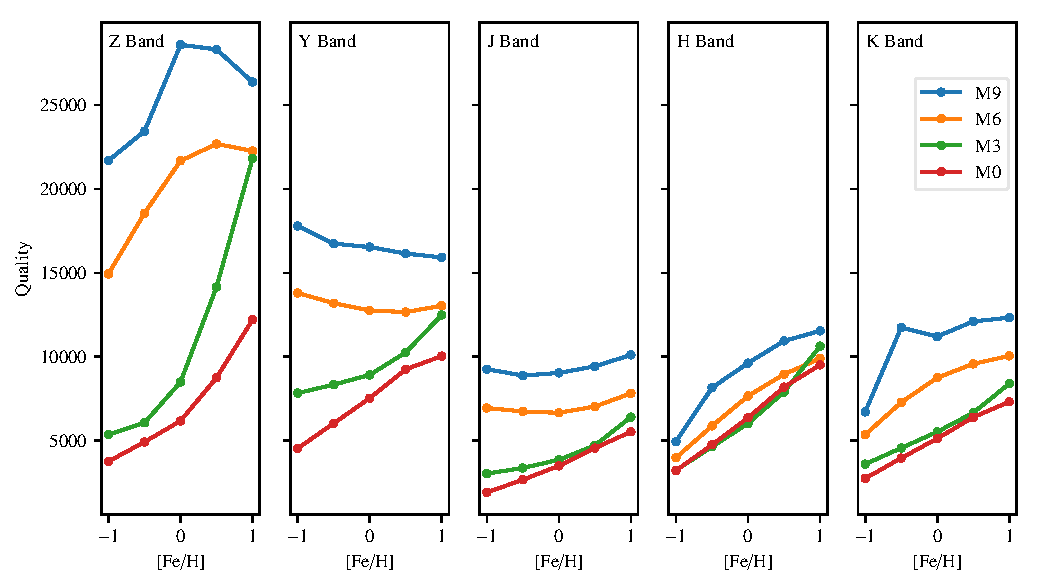
\includegraphics[width=0.99\linewidth]{figures/information-content/metalicity_effect.pdf}\\
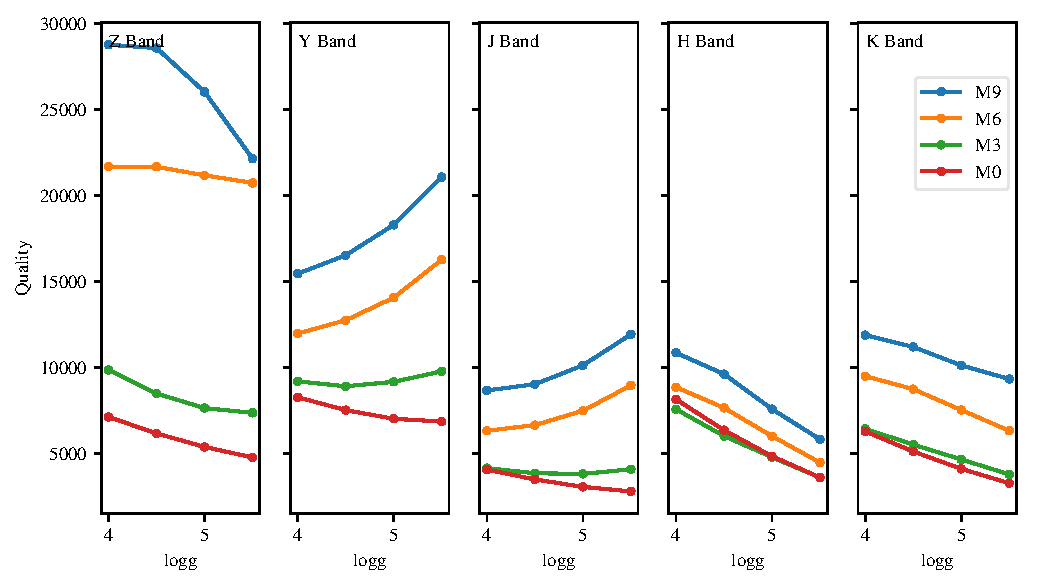
\includegraphics[width=0.99\linewidth]{figures/information-content/logg_effect.pdf}
\caption[Quality factor verse \feh{} and \Logg{} for different spectral types and wavelength bands.]{Quality factor changes across spectral type and bands for variations in \feh{} and \Logg{}.
Broadening values are R=100\,000 and \Vsini{}=1.0\kmps{}.
Top: Quality factor variation of \feh{} between -1.0 to 1.0 at a fixed \Logg{}=4.5.
Bottom: Quality factor variation of \Logg{} between 4 and 5.5 with fixed \feh{}=0.0.
Note a higher quality factor corresponds to an increased {RV} precision.}
\label{fig:deviations}
\end{figure}


\clearpage

\section{Updating {RV} precision software}
To undertake the calculation of {RV} precisions
A large section of this work involved optimizing the original code used in~\citet{figueira_radial_2016}.
Care needs to be taken to optimize the code.
The original code used in~\citet{figueira_radial_2016} was slow, taking around 2 hours per simulation, this led to multiple weeks of processing time to compute the precision's for the original paper.

In this section \todo{we} document the changes made to the code in the course of attempting to improving it.
Features that change the derived {RV} precision are specifically documented in detail, with relative precision changes provided.

This work resulted in a submission of a publication\footnote{Available at \href{http://joss.theoj.org/papers/384bfc031df47ecef2d88328f63e5479}{http://joss.theoj.org/papers/384bfc031df47ecef2d88328f63e5479}} to \emph{The Journal of Open Source Software}\footnote{\href{http://joss.theoj.org/}{joss.theoj.org/}} (JOSS) {Neal and Figueria 2018 (in prep.)} with the source code openly available on \href{Github}{https://github.com/jason-neal/eniric}.


\subsection{Automated testing}
To insure that any changes made to the code did not change the underling results.
This involved writing automatic tests for the software.
This practice is crucial in computer science ins commercial software development but seldom done in research but is becoming more popular.
\reference{works of software testing in research.}
Some work focused on testing ideology from computer science.
Although not perfect implementation I began by adding automated tests to the code to check individual parts of it.
Before making changes I created automated tests that would confirm the functionality of pieces of the code.
I could then make changes to the code, to improve the performance without worrying that the results were different.
Namely that the same precision were calculated in the end.

Functional test and unit tests.


\subsection{Performance}
\label{subsec:code_performance}
There was a major performance bottleneck in the convolution stage, which increased the performance around 250\,X itself.
The algorithm looped though the pixels in the spectrum, selecting out the necessary section around a given pixel with a comprehension list (for loop if inside range).
Turning the result into a \emph{numpy} array, performing the sum for that pixel and appending it to a list.
The performance issue was a python implementation detail to do with applying a comprehension list to a \emph{numpy} array, then slicing the \emph{numpy} array with the ends of the list, then converting it back into a \emph{numpy} array, all of which is performed on a very large spectrum array.
Creating a \emph{numpy} boolean mask instead of the comprehension list, and applying the boolean mask to the array is much faster.
Remaining entirely in the compiled \emph{numpy} code and not converting between lists and \emph{numpy} arrays (with involve type checking overhead).
This slow operation was done for every pixel/wavelength in the spectrum twice, once for each convolution.

caching convolution result to prevent recomputing the same values with \emph{Joblib}.
Also embarrassingly parallel so added multiprocessing support.

The convolution is still the slowest part.
There are other methods that work on uniform spectra, which have not been tried to see how they affect the performance or {RV} precision results.
\textbf{Insert code samples.}


\subsection{Model extension}
The solution is to iterate over each pixel but create a mask array and use \emph{numpy} indexing to select the required pixel span.
(this remains in \emph{numpy})
These operations all remain in \emph{numpy} so do not waste time converting between lists and \emph{numpy} arrays, in which Python need to constantly check and convert the type of each item.

This shows a lesson in the usefulness of test driven development, or testing of code in science.


An normalization step was originally done after the convolution, to normalize out the effect of the convolution on a spectrum of 1s, due to the changing wavelength grids sampling.
This was brought inside the main convolution by dividing the pixel by the convolution of a spectrum of ones at the same time.
 (again in \emph{numpy} so it is quick)

Parallelization as embarrassingly parallel, the result of each pixel is independent of result of neighbours.

This is not a criticism of the work done by the original author (my supervisor).
It is easier to modify a working system then to create one from scratch.

Computer code is not the important part in scientific exploration., although becoming more important in open source and reproducibility efforts.
Often forgotten in

\# Handle any {PHOENIX} aces models.


\section{Numerical Gradient}
\label{sec:numerical_gradient}
One of the key insights from \cref{eqn:optimal_weight,eqn:dv_rms} is that the radial velocity error is inversely proportional gradient of the spectra, In numerically computing the {RV} precision, the result is dependent on the numerical method used to compute the gradient.
In original code used in~\citet{figueira_radial_2016} the gradient or slope is approximated using the forward finite difference method.
The \emph{numpy} package provides a function to calculate the gradient using a more advanced methods that compute a more precise gradient.
In this section \todo{we} explore the affect of improving the precision of the numerical gradient on the final {RV} precision.

The simplest way to calculate the derivative using finite difference methods~\citep{quarteroni_numerical_2000}.
These arising from the Newton's definition of the derivative for a continuous function \(f(x)\) which should be familiar from introductory calculus:
\[f'(x) = \lim_{h \to 0} \frac{f(x+h)-f(x)}{h}~.\]

There are three common varieties of the finite difference,
\begin{equation}
 {FFD} = \frac{f(x+h)-f(x)}{h}, {CFD}=\frac{f(x+\frac{1}{2}h)-f(x-\frac{1}{2}h)}{h}, {BFD}=\frac{f(x)-f(x-h)}{h}\,,
\end{equation}
called the forwards ({FFD}), central ({CFD}), and backwards ({BFD}) finite differences respectively.
The order of uncertainty on the {FFD}/{BFD} is \(\mathcal{O}(h)\) while for the {CFD} it is \(\mathcal{O}({h}^{2})\)~\citep{quarteroni_numerical_2000}.
As the wavelength spacing between samples/pixels (h) is small the {CFD} will a more precise value for the gradient at each pixel.

In this case \(h\) is the difference in wavelength between the two pixels considered.
In the {FFD} case the gradient at pixel \(i\) becomes:
\begin{equation}
\frac{\partial A_0(i)}{\partial\lambda(i)} = \frac{A_0(i+1) - A_0(i)}{\lambda(i+1)-\lambda(i)}, \hspace{2em} 1 \leq i \leq n-1.
\label{eqn:ffd_precision}
\end{equation}
At each pixel the numerical derivative is evaluated to be the average slope between itself and the following pixel and is an approximation to the derivative.
This only extends to \(i= n-1\), where \(n\) is the number of points in the spectrum, and the last pixel is dropped from the {RV} calculation.\footnote{This is important in the case of Condition~\#2.}


The \emph{gradient}\footnote{Documentation available at \href{https://docs.scipy.org/doc/numpy/reference/generated/numpy.gradient.html\#id1 }{https://docs.scipy.org/doc/numpy/reference/generated/numpy.gradient.html\#id1}}  method provided in \emph{numpy} contains a more advanced numerical methods to calculate the derivative.
It uses a \textit{compact difference} method~\citep{quarteroni_numerical_2000} which expand the finite differences using a Taylor expansion and then selecting coefficients to minimize the \textit{consistency error}.
From the \emph{numpy} documentation the consistency error here is \[\eta_i = \partial{f(x_i)}/\partial{x} -  [\alpha f(x_i) + \beta f(x_i +h_d) + \gamma f(x_i - h_s)],\] where \(h_s\) and \(h_d\) are the spacing to the left and right of \(i\) respectively.
With Taylor expansion this turns into solving a linear system of equations:
\[\begin{cases}
         \alpha + \beta + \gamma = 0\\
         -\beta {h_d} + \gamma {h_s} = 1\\
         \beta {h_{d}}^{2} + \gamma {h_{s}}^{2} = 0
    \end{cases}
\]
which result in the approximation of the gradient of the central values to be

\[\frac{\partial{f(x_i)}}{\partial{x}} = \frac{{h_{s}}^{2}f\left(x_{i} + {h_{d}}\right) + \left({h_{d}}^{2} - {h_{s}}^{2}\right)f\left(x_{i}\right) - {h_{d}}^{2}f\left(x_{i}-{h_{s}}\right)} {{h_{s}}{h_{d}}\left({h_{d}} + {h_{s}}\right)} + \mathcal{O}\left(\frac{h_{d}{h_{s}}^{2} + {h_{s}}{h_{d}}^{2}}{{h_{d}} + {h_{s}}}\right) \label{full_compact_difference}.\]

If the spectrum is evenly spaced ${h_{s}}={h_{d}}$  reduces to the standard second order {CFD} approximation:

\[\frac{\partial{f(x_i)}}{\partial{x}} = \frac{f\left(x_{i+1}\right) - f\left(x_{i-1}\right)}{2h} + \mathcal{O}\left({h}^{2}\right)\]


Applying this to the situation presented here, similar to \cref{eqn:ffd_precision}, results in:
\[\frac{\partial A_0(i)}{\partial\lambda(i)} = \frac{{\lambda(i-1)}^{2} A_0(i+1) + ({\lambda(i+1)}^{2}-{\lambda(i-1)}^{2}) A_0(i) - {\lambda(i+1)}^{2} A_0(i-1)} {\lambda(i-1)\lambda(i+1)(\lambda(i+1) + \lambda(i-1))}, \hspace{1em} 2 \leq i \leq n-1\]

with an uncertainty of \(\mathcal{O}\left(\frac{\lambda(i+1){\lambda(i-1)}^{2} + \lambda(i-1){\lambda(i+1)}^{2}}{\lambda(i+1) + \lambda(i-1)}\right)\).


{\red{} Wavelength spacing \(\delta\lambda\) between pixels is a function of \(\lambda\), Resolution and sampling choices.
Can I do something with this??}

The \emph{gradient} function from \emph{numpy} implements central differences for the interior points, accurate to second order, and first order accurate one-sided (forward or backward) differences at the boundaries, computed using the same compact difference procedure.

\begin{figure}
    \centering
    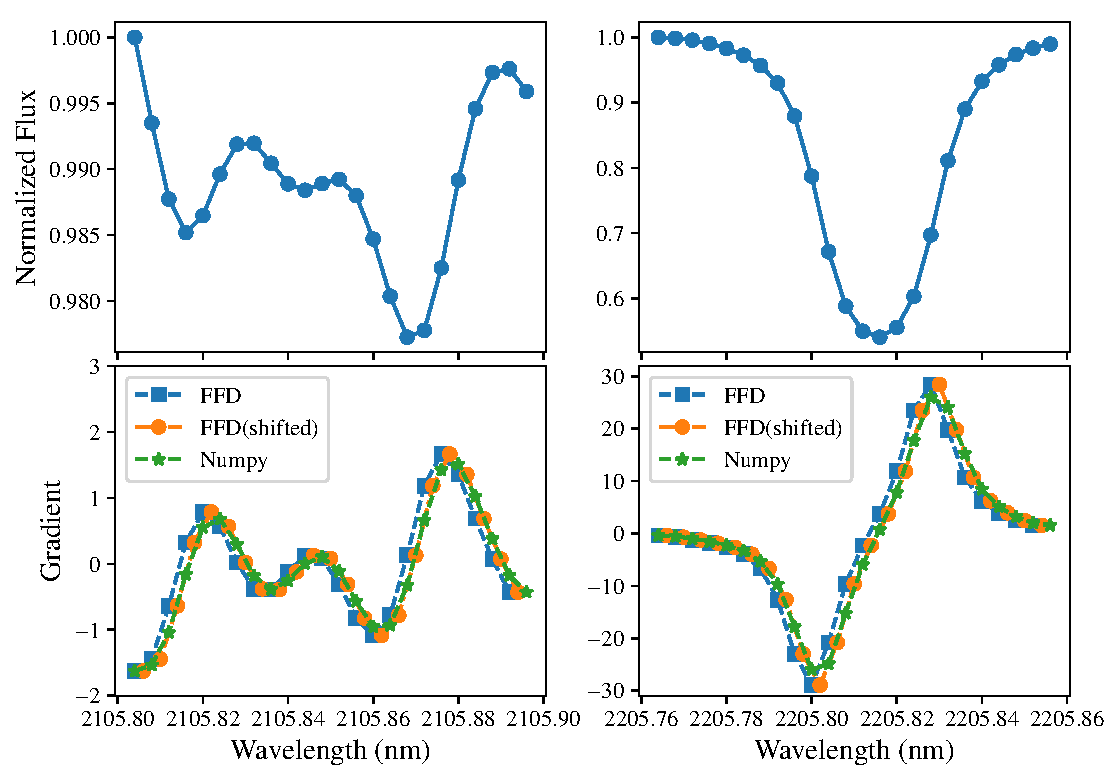
\includegraphics[width=0.8\linewidth]{figures/information-content/spectral_gradients}\\
    \caption[Comparing of numerical gradient alogithms.]{Visualization of the numerical gradient of some spectral lines.
        Top: The two spectral regions of a stellar spectrum the left hand slide contains short lines near the normalized continuum while on the right a single deep absorption line is shown.
        Bottom: The numerical gradients for the spectra shown in the top panels; the original {FFD} method is displayed with \emph{blue squares} while \emph{numpy} gradient is shown with \emph{green stars}.
        The \emph{orange circles} are the {FFD} version shifted to the mid-points between pixels for illustrative purposes.}
    \label{fig:gradients}
\end{figure}


%!TEX root = ../thesis.tex

\begin{table}
    \caption{The affect of the numerical gradient function on RV precision. The band label \(\rm VIS\) indicates the visible band while  \(\rm CARM_{VIS}\)  and \(\rm CARM_{NIR}\)  indicate the two wavelength bands of the CARMENES spectrograph. \(\Delta\lambda\) is a wavelength shift applied to analyse the pixel weights at the middle of their FFD gradients for comparison only.}
    \begin{tabular}{ccccccc}
        \toprule
%% Band & $\lambda$ range\_min & wl\_max &  dy/dx   & gradient & Q(dy/dx) & Q(grad) & Q(frac) & RV(dy/dx) & RV\_adj &    RV(grad)    &    RV(frac\_grad)    & RV(frac\_adj)          \\
  &   $\lambda$ range & \multicolumn{3}{c}{RV\(_{rms}\) (\mps{})} & \(\Delta\) RV ratio& \(\Delta\) RV ratio\\
 Gradient method&  &  A &   B & C & (B-A)/A & (C-A)/A \\
 Band  &  \si{\micro\meter} & FFD & FFD+\(\Delta\lambda\) &  CFD &  \% & \% \\
    \midrule
VIS & 0.38 -- 0.78 & 16.1 & 16.2 & 16.9  & 0.6 & 4.9\\
\(\rm CARM_{VIS}\) & 0.52 --  0.96 & 20.9 & 21.0 & 22.0 & 0.3& 5.2 \\
Z & 0.83 -- 0.93 & 76.9 & 77.0 & 78.8  & 0.1 & 2.5\\
Y & 1.00 -- 1.10 & 78.3 & 78.5 & 83.8 & 0.2 & 7.0 \\
J & 1.17 -- 1.33 & 149.3 & 149.4 & 156.4 & 0.1 & 4.7 \\
H & 1.50 -- 1.75 & 119.4 & 119.5 & 122.3 & 0.1 & 2.5 \\
K & 2.07 -- 2.35 & 153.4 & 153.7 & 157.7  & 0.2 & 2.8\\
\(\rm CARM_{NIR}\) & 0.96 -- 1.71 & 46.1 & 46.2 & 48.0 & 0.1& 4.2 \\
NIR & 0.83 -- 2.35 & 36.9 & 36.9 & 38.2 & 0.1 & 3.6  \\
    \bottomrule
    \end{tabular}\label{tab:numerical_gradients}
\end{table}


In \cref{fig:gradients} \todo{we} visualize the gradients of two small spectral regions computed with the original {FFD}, and the higher precision version incorporated in numpy's gradient function.
The top panels contain the spectrum in the small regions shown, indicating a large spectral line and three small lines near the continuum respectively.
The derivative of the spectra is shown in the bottom panel with the {FFD} method shown with \emph{blue squares} and the \emph{numpy} gradient shown in \emph{green stars}.
The \emph{orange circles} are the same as {FFD} but shifted horizontally to the midpoints between pixels.
This is for illustrative purposes and to assess the effect of this offset when calculating the pixel weights.

There a three notable features observed between gradient methods.
The first, which is expected from the {FFD} formulation is that the {FFD} gradient is offset to the left.
The second is that when the horizontal offset is adjusted (orange circles) the gradients lie along the same curve.
Both methods are trying to approximate the real gradient function of the spectrum and is again expected.
The most important feature observed in this though is that there is a slight over-estimate of the gradient by the {FFD} method at the peaks.
In the bottom panels of \cref{fig:gradients}, the points of highest gradient are always from the {FFD} method (blue/orange).
This is the case for all spectral lines and as the optimal pixel weights are proportional to the gradient squared the {FFD} method will apply slightly higher pixel weights to these values, two points per line in the spectrum.
The {FFD} will therefore produce a slightly smaller \(\delta V_{\rms}\) error compared to the more precise gradient function.

In \cref{tab:numerical_gradients} \todo{we} calculate the  \(\delta V_{\rms}\) using both gradient methods to determine their relative effect on the {RV} precision.

We took a {PHOENIX-ACES} spectrum with \Teff{}=3900\K{}, corresponding to {{M0}} spectral type.
The full theoretical precision is calculated (no telluric masking applied) with no rotational or instrumental broadening and the maximum of the continuum of each band scaled to 1.
In this case the {RV} precisions are not comparable between bands and are only to assess the direct effect of the changing the numerical gradient.
The bands name and the spanned wavelength are given.
The columns A, B, C are the {RV} precision for the different gradient methods.
The \(\delta V\) ratios are the relative difference in {RV} when changing from method A (the original {FFD}) to methods B and C.
In this table column B is the {FFD} method but with the wavelength shifted to in between pixels, corresponding to the orange circles in \cref{fig:gradients} while column C is the more precise gradient from numpy.

We find that changing to use the gradient from \emph{numpy} increases the \(\delta V_{\rms}\) by 2.5--7\%, (decreasing the {RV} precision), due to the over-estimated gradient from the {FFD} method.
As the pixel weights \cref{eqn:optimal_weight} are also proportional to \({\lambda}^{2}\) column B was computed to assess the effect of the slight wavelength offset on the {RV} precision, visible in \cref{fig:gradients}.
This small wavelength shift red-ward does changed the {RV} precision by 0.1--0.6\% which is an order of magnitude smaller than the relative change when using numpy's gradient method.

Changing the method of numerical derivatives will change all the precision values given in the~\citet{figueira_radial_2016}.
This is a small impact on on the precision compared to other components of the {RV} precision.
For instance from \cref{eqn:rv_SNR} a increase in \(\delta V_{\rms}\) of between 2.5--7\%  could equally be caused by a small decrease in the \snr{} from 100 (the value used in~\citet{figueira_radial_2016}) to between 95--98.

The current version of the software is now implemented with the gradient method provided by \emph{numpy} package.

\subsection{Masking Function}
\label{subsec:masking_function}
Another change made to the software is in the application of the masking function, and the treatment of telluric lines.
As suggested in~\citet{connes_absolute_1985} and~\citet{bouchy_fundamental_2001} a custom masking function can be applied to the individual pixel weights in \cref{eqn:optimal_weight}, such as:

\[W'(i) = W(i)M(i),\label{eqn:mask_function}\] where \(M(i)\) is the masking function and \(W'(i)\) are the modified pixel weights.
This masking function can be used in particular for the removal of telluric lines, setting those weights to zero and is in essence what is done when wavelength selection is performed; assigning zero weight to all pixels outside the desired wavelength range.

This masking function can be used to easily apply the three conditions presented in~\citet{figueira_radial_2016}.
First the 3 masking functions will be defined, then followed by the quantification of how they differ from the previous implementation.
The subscripts on the masking functions correspond to the three conditions.
\begin{align}
M_1(i) &= 1 \label{eqn:mask1}\\
M_2(i) &= \begin{cases}
0, \hspace{1em} T(i) < \tau\\
1, \hspace{1em} T(i) \ge \tau\\
\end{cases}\label{eqn:mask2}\\
M_3(i) &= {T(i)}^{2} \label{eqn:mask3}
\end{align}

Here, \(T(i)\) is the telluric transmission spectrum, while \(\tau\) is the transmission depth cut-off.
For instance to mask out telluric lines deeper than 2\%,  \(\tau\) would be set at 0.98.

\begin{itemize}
    \setlength\itemsep{-0.2em} % Remove spacing on list.
    \item Condition~\#1:
    The first mask, \(M_1\), is the simplest case in which all pixel weights are treated equally.
    No telluric line masking is considered.

    \item Condition~\#2:
    In the second mask, \(M_2\), the telluric line transmission, \(T(i)\) is used to create a boolean mask of 0's and 1's.
    When applying this mask to the pixel weights, the pixels effected by telluric lines have 0 weight, removing their contribution to the {\red{} \(RV_{\rms}\)}.
    Accounting for seasonal variation in Earth's barycentric motion can be easily incorporated into this mask, widening the regions masked out.

    \item Condition~\#3:
    The third mask, \(M_3\), assumes the application of perfect telluric correction consistent with Condition~\#3.
    The pixel weights are modified by dividing the flux variance by the square of the transmission spectrum\reference{cite the equation when I refer to it}.
    As the flux variance is the denominator of \cref{eqn:optimal_weight}, this is equivalent to multiplication of the weights by a mask of the form \(M_3\).
\end{itemize}

Having the three masks defined in this way makes the implementation of the {RV} precision simpler.
In the original version there were three separate implementations, one for each condition.
With this, \todo{Check this if it is previous}{as mentioned previously} there was a issue with the implementation of Condition~\#2.

\subsubsection{Masking order}
\label{subsubsec:masking_order}
The order in which the masking is performed is also important.
Masking should be applied only after calculation of the pixel weights.
As the pixel weights depend on neighbouring points (through the calculation of the gradients), prematurely removing pixels will affect the precision results.

The original implementation of Condition~\#2 did just this, splitting the spectra into small sections in between the masked off telluric lines.
The {\red{}\(RV_{\rms}\)} is calculated for each section and then the results are combined as the error on the weighted average in \cref{eqn:weighted_average_error}.
Analytically this identical to masking the pixel weights with \(M_2\) but not in practice when numerically implemented.
\todo{Should I show the working of analytical working out of this in an appendix, or here?}

When the spectrum is split into small sections the number of edges increases and the number of pixels affected by any edge effects increases.
Using the {FFD} method to compute the gradient the last pixel is removed/lost.
A spectrum split in \(m\) sub-spectra will therefore lose \(m\) pixels due to edge effects (instead of only 1 pixel with the full spectrum).
Even the \emph{numpy} gradient is not immune to the edge effects in the sub-spectra when splitting the spectrum first.
Even though there is no pixels lost, the first and last pixels of each sub-spectra are computed using forward or backward differences, rather than central differences (as they would be in the full spectrum).
Hence the gradients and weights of some pixels are slightly changed due to the splitting occurring first.

We quantify the effect of splitting the spectrum before and after calculating the weights in \cref{tab:mask_ordering}.
The columns label \emph{Split} represents splitting the spectrum before calculating the pixel weights while the \emph{Mask} columns calculate all the pixel weights first and then apply the \(M_2\) mask.
The difference in {RV} precision between both situations and for both gradient methods are given.
For the {FFD} gradient the ordering of masking changes decreases the {\red{}\(RV_{\rms}\)} by 0.2--0.7\%, while for the \emph{numpy} gradient it is increase but an order of magnitude smaller between 0.01--0.13\%.
The {FFD} gradient is causes a larger difference as points that were masked out are now included where as with the \emph{numpy} gradient the end values are always included but their gradients are slightly changed.
The last column is the difference ratio between the \emph{Mask} column of both gradient method, this is consistent with \cref{tab:numerical_gradients} with the differences from two gradient methods between 2--7\%.
It shows that the difference from changing order of masking is 1--2 orders of magnitude smaller than changing the gradient method.

The code has been adjusted to consistently apply the masking after the pixel weights are calculated.
This retains the most pixels, with the more accurate pixel weights.
It has also been changed to just apply \(M_2\) rather than splitting and performing the weighted error calculation.
\todo{did I check this was equivalent} This simplifies the implementation in calculating the {RV} precision.

%!TEX root = ../thesis.tex

\begin{table}
    \centering
    \caption{Relative {RV} precision difference for Condition \#2 due to spectral splitting and order of applying the pixel mask. The ratio are the difference between Split and Masked implementations with the same gradient calculation. The last column is the ratio between the Masked versions using the FFD and numpy gradient methods and are consistent with \tref{tab:numerical_gradients}. Results a for an M0 spectral type, with vsini=1.0 and R=100,000.}
    \begin{tabular}{c|ccc|ccc|c}
        \toprule
        & Split & Masked & \(\Delta\)Ratio & Split & Masked & \(\Delta\)Ratio & Masked \\
        Gradient & \multicolumn{3}{c|}{FFD} & \multicolumn{3}{c|}{Numpy} & \(\Delta\)Ratio\\
        Band & \mps{} & \mps{} &  \%  & \mps{} & \mps{} &   \% & \% \\
        \midrule
        Z &  7.42 &  7.38 & -0.66 &  7.76 &  7.77 & 0.13 & 5.3\\
        Y &  4.75 &  4.74 & -0.22 &  5.06 &  5.06 & 0.06 & 6.8\\
        J & 18.58 & 18.53 & -0.29 & 19.57 & 19.57 & 0.01 & 5.6\\
        H &  6.08 &  6.05 & -0.53 &  6.25 &  6.26 & 0.08 & 3.5\\
        K & 32.21 & 32.14 & -0.22 & 33.48 & 33.49 & 0.05 & 4.2\\
        \bottomrule
    \end{tabular}\label{tab:mask_ordering}
\end{table}

{\rd{} The results from these spectra for conditions \#1 and \#3 are consistent with Figueira et al. 2016. \todo{put this some where}}


{\red{} For Condition~\#2 in which there was an error there is no meaningful relation between the new and old values.
\todo{put this line elsewhere.}}


\subsection{Atmospheric masking bug}
\label{subsec:condition_two_bug}
One thing that was revealed in testing was that there was an error in the application of Condition~\#2.
When the telluric mask was shifted to account for barycentric motion of the earth, and the condition of 3 consecutive pixels in the telluric spectra being lower than the limit (due to the higher sampling) there was an software bug,


A check for this issue was discovered using this unit test.
\begin{lstlisting}[language=Python, caption=Example unit test to catch masking bug. The assert statement checks that the mask continues to remove all absorption lines deeper than 2\%.]
def test_telluric_masking(wavelength, transmission):
    """Check mask still masks out all telluric lines > 0.98 after
    accounting for barycentre motion."""
    mask = telluric_mask(transmission, depth=0.98)  # Create mask
    mask = barycentre_shift(wavelength, mask)       # Extend mask
    assert numpy.all(transmission[mask] >= 0.98)    # Check mask
\end{lstlisting}
The assert statements checks that when the mask is applied to the transmission spectrum again all of the values are outside of any deep telluric regions.
A test like this would have caught this bug.

This bug means that all the {RV} precision values for Condition~\#2 published in~\citet{figueira_radial_2016} incorrect.
As the applied masking was unevenly applied~\citet{figueira_radial_2016} the new values {RV} precision values do not all change in the same proportion or direction.
Some specific wavelengths and resolutions are essentially unchanged while other results change by over 20\mps{}.
Even though there is an error with condition~\#2 they do not change the overall conclusions of the paper.
These are \todo{add conclusions not affected}

\subsection{\snr{} scaling}
\label{subsec:snr_scaling}
To analyse the relative precision of different spectra they need to normalized to a common reference point.
In this section \todo{we} detail how this was originally done and how this was changed to be adaptable to any library spectra and any reference band.

In the original code this was selected to be a \snr{} per pixel of 100 at the centre of the \textit{J}-band at 1.25\si{\micro\meter}.
The normalization values for each band, \Vsini{} and resolution combination were hard-coded into the analysis.
This made it impossible to easily adapt the code to other spectra or parameter combinations.

An automated \snr{} scaling procedure was created to remove the hard-coded values.
This updated code finds the centre point of the band of reference for the given spectrum.
Totals the photon count across one resolution element, \(\delta\lambda\), and then takes the square root.
This is using the definition of the \snr{} as \(\snr{} = \sqrt{N}\) for large N.
This value is then used to scale the spectrum such that the \snr{} at the reference point is the desired value.
\begin{equation}
    SF =  \frac{\sqrt{\sum{\delta\lambda} A}} {\snr{}_{desired}}
\end{equation}
\textit{SF} where \textit{SF} is the scaling factor, \(\sum_{\delta\lambda} A\) is the sum of the point in one resolution element and \({\snr{}}_{desired}\) is the desired \snr{} level requested.

This automated procedure enabled {\red{}\textbf{4}} different features.
\begin{itemize}
    \setlength\itemsep{-0.3em} % Remove spacing on list.
    \item The ability to analysis other spectral models, not just corresponding to {M0}, {M3}, {M6}, {M9} spectral types.
    - Scaling to a \snr{} per pixel level other than 100.
    \item A \snr{} per pixel other than 100 can be selected.
    - Allowing for other sampling levels (if desired)
    \item Not restricted to a model with 3 samples per resolution element.
    \item Different reference bands available.
    Results are not limited to being referenced from the \textit{J}-band.
    For instance the {RV} precision can now be calculated for a given \snr{} at the centre of the \textit{K}-band.
    This was one the features requested for the Exposure Time Calculators precision values.
    For {NIRPS} \todo{we} provided precision values relative to each individual band, while for {SPIRou} they were relative to the {J}- and {H}-bands.
\end{itemize}

The default values for the \snr{} scaling a still 100 at the centre of the \textit{J}-band, but there is now options to easily change these values.

The centre of each band was visually checked to ensure that there were no spectral lines at the reference locations> If a line was present at the reference point its depth variability across spectral types would affect the \snr{} scaling levels at a greater than the normal change in continuum amplitude/shape.\todo{is this needed}

As shown in \cref{eqn:snr_relation} the {RV} precision is inversely proportional to the \snr{} level.
To access the {RV} precision of any of the values in Table at a different \snr{} level you can apply the following
\begin{equation}
\rm {RV}_{\snr{}2} = {RV}_{\snr{}1} * \frac{\snr{}1}{\snr{}2}.
\end{equation}

\todo{\snr{} plot/diagram}
\section{{SPIRou} and {NIRPS} {ETC}}\label{sec:spirou_nirps_etc}
Having this tool to calculate {RV} precisions efficiently lead to contributions to the Exposure Time Calculators (ETC) for both the {SPIRou} and {NIRPS} spectrographs.

In September 2017 \todo{we} were requested to provide precision calculations for the {SPIRou} ETC\footnote{\url{http://www.cfht.hawaii.edu/Instruments/SPIRou/SPIRou_etc.php}}.
These were the same table as~\citet{figueira_radial_2016} but with a each band referenced to 100~{\snr{}} in its own band.
The modification to use the centre of any band was made to fulfil this request.
Notes on the telluric correction issue affect on Condition~2.

In May 2018 \todo{we} were requested to provide precision calculations for the {NIRPS} {ETC}.\@ This extended the spectral range from {M0}, {M3}, {M6}, {M9} at 3900, 3500, 2800, 2600\K{} respectively, but to all temperatures between 2500 and 4000\K{} inclusively.
This provides a finer resolution coverage over the M spectral type, allowed by the {PHOENIX-ACES} library.
Instrumental resolutions of 75\,000 and 100\,000 were requested to match the {NIRPS} instrument.
The \Logg{} and metallicity, sampling rate remained at the~\citet{figueira_radial_2016} levels of 4.5, \textbf{0.0} and 3.0 respectively.\todo{}
Precisions were provided for \snr{} of 100 relative to the \emph{J}-, \emph{H}-bands as well as to each band individually.
Artigua 2018 (private communication 2018).\todo{Check how to cite priv communication properly}  suggested the truly relevant value is the \snr{} in \emph{H}-band for {NIRPS} radial velocities.

The results can be manually generated using ``eniric'' with the following incantation (after installation and configuration of {PHOENIX} library spectra.)
\textbf{A table of the precisions created for the {NIRPS} ETC are provided as an online table to \todo{our} publication} {Neal et al.
2018b (in prep.)}\footnote{Review at \href{https://github.com/openjournals/joss-reviews/issues/1053}{https://github.com/openjournals/joss-reviews/issues/1053}} \todo{Fix up when accepted}.


These values were both calculated and provided using the {FFD} gradient and with the incorrect masking order for Condition~\#2, splitting before calculating the pixel weights.
As \todo{we} demonstrated in \cref{sec:numerical_gradient,subsubsec:masking_order} these have a {RV} precision \(\sim\)2--7\% better than what would be computed with the current implementation.


\section{ Updated Figueira 2016 results}
\todo{comparison of plots} figueira eta la plot 1, eniric plot

\begin{figure}
    \centering
    \begin{tabular}{cc}
    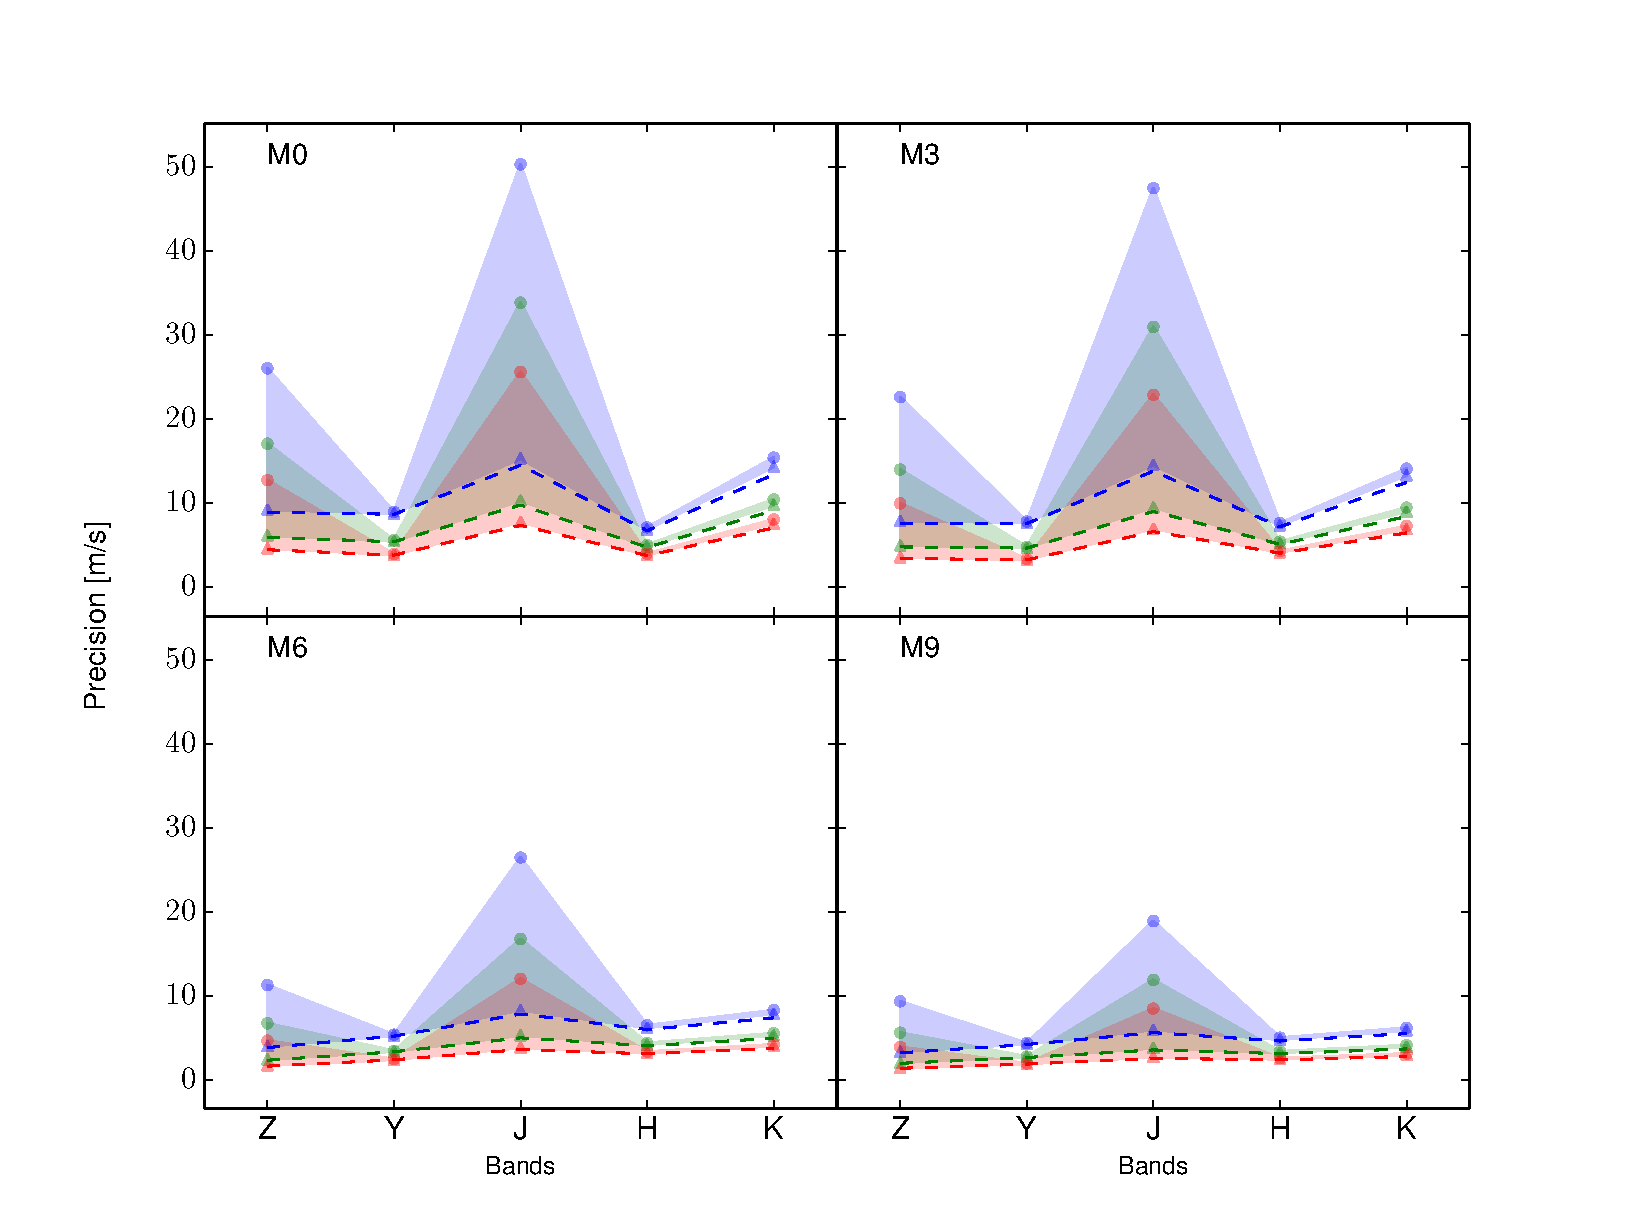
\includegraphics[width=0.48\linewidth]{figures/information-content/Rvprec_vsini1.pdf} &  % Figueria plot
    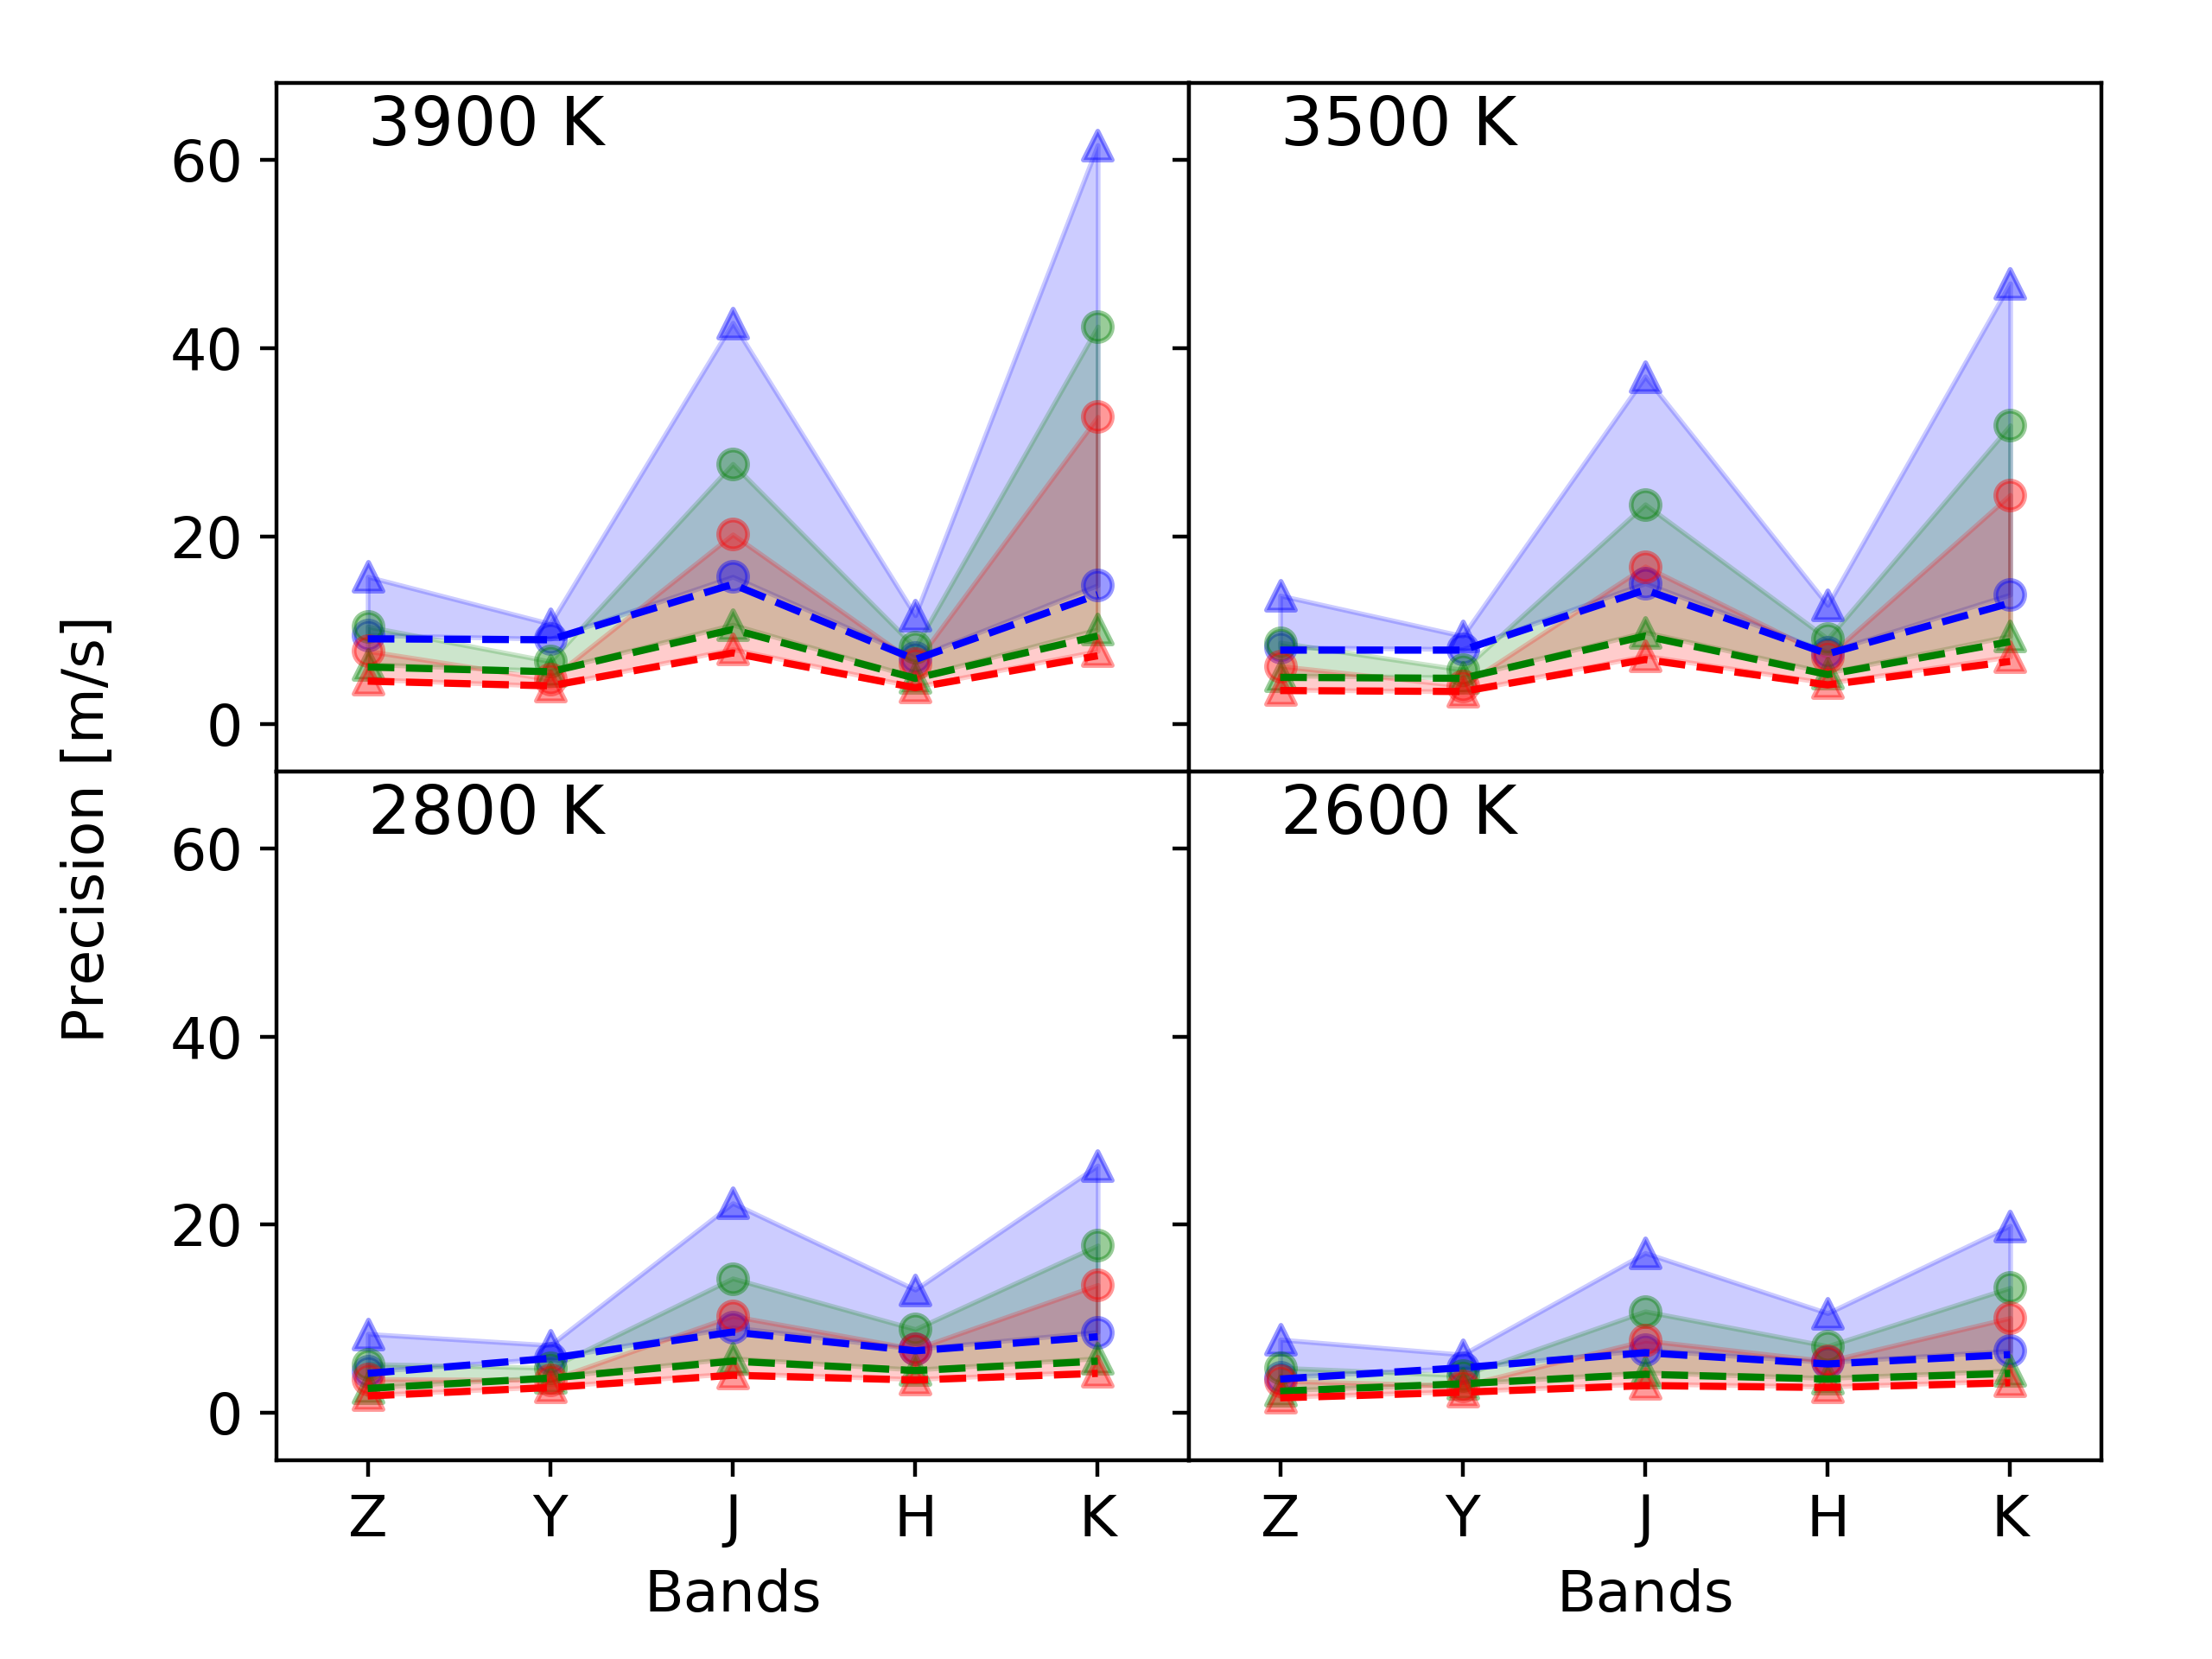
\includegraphics[width=0.47\linewidth]{figures/information-content/precision_fourpanel.png}\\ % eniric plot
    \end{tabular}
    \caption[Comparision of {RV} precision results to~\citet{figueira_radial_2016}.]{Left: Figure 1 from~\citet{figueira_radial_2016}.
        Right: The same style figure with values updated from this work, computed with \emph{eniric}.
        The main difference is the area of shaded region due to the problem with Condition~\#2 (which is the upper edge).}
    \label{fig:my_label}
\end{figure}
\todo{Change to 55\mps{} upper limit?}

\section{ metalicity / \Logg{} extension}



%!TEX root = ../../thesis.tex

\section{Application to {CARMENES} spectra}

One of the main reasons for focusing on extending the work of~\citet{figueira_radial_2016} was to analyse the differences in {RV} precision of synthetic spectra and observed \nir{}.
This is important for the community to understand the accuracy of synthetic spectra.
\citet{artigau_optical_2018} recently found band-specific discrepancies in the theoretical precision between real and synthetic \nir{} spectra of Barnard's Star.
In 2018 {CARMENES} openly released a spectral library containing one spectrum for each target in their 324 M-dwarf {RV} survey in~\citet{reiners_carmenes_2018}.
With this they provide details on the empirical \(\delta V_{rms}\) measured during their {RV} processing with their {RV} analysis code, {SERVAL}~\citep{zechmeister_spectrum_2018}, using all available spectra of each target.
Spectra from this library has been used to compare the theoretical precision of observed {CARMENES} spectra to synthetic models, and is still in the preliminary stages, with the progress so far demonstrated here.

\subsection{Target selection}
\label{subsec:carmense_targets}
To analyse the precision in different spectral types, a few specific M-dwarfs were selected.
These were selected from the 324 spectra of the {CARMENES} M-dwarf library from~\citet{reiners_carmenes_2018}\footnote{Available at \href{http://carmenes.cab.inta-csic.es/gto/}{\url{http://carmenes.cab.inta-csic.es/gto/}}.}, along with the achieved \snr{} in the visible and \nir{} spectra.

The spectral library data was downloaded, divided into spectral type and ordered by the stated \nir{} {SNR}, to select targets at the high \snr{} end.
To cover the M-dwarf range, targets were selected near each of the spectral types M0, M3, M6 and M9.
For each spectral type (within $\pm0.5$) two stars are selected that have high {SNR} values. This will give eight spectra over the M-dwarf range to analysis.
One of the two selected targets for the M3 type is Barnard's star which has been analysed extensively in~\citet{artigau_optical_2018}, in particular with CRIRES spectra for the \nir{} domain, allowing for direct comparisons between the two works.
The other criteria used for selection was to select targets with a varied range of \Logg{} and \feh{} values if possible.

The selected targets from the {CARMENES} library are provided in \cref{tab:carmenes_selection_updated}.
The spectral parameters (\Teff{}, \Logg{}, \feh{}) for these targets are from~\citet{passegger_carmenes_2018, rajpurohit_exploring_2018} who performed spectral fits of the {CARMENES} spectra with the {PHOENIX-ACES} and {BT-Settl} models respectively.
The uncertainties in the~\citet{rajpurohit_exploring_2018} parameters are \(\sigma_{\teff{}}\)=100\K{}, \(\sigma_{\logg{}}\)=0.3, and \(\sigma_{\feh{}}\)=0.3 while the uncertainties on the 
\citet{passegger_carmenes_2018} values are \(\sigma_{\teff{}}\)=51\K{}, \(\sigma_{\logg{}}\)=0.07, and \(\sigma_{\feh{}}\)=0.16.
There are gaps in the~\citet{passegger_carmenes_2018} values for stars that have the lower \snr{} levels as they are more difficult to analyse/fit.
Neither one has parameters for Luyten's Star, for which the parameters given are from {SIMBAD}.

\begin{landscape}
    %!TEX root = ../../thesis.tex

\begin{table}[h]
    \centering
    \begin{threeparttable}
        \caption[{CARMENES} targets for {RV} precision analysis.]{Selected {CARMENES} targets with stellar parameters from both~\citet{rajpurohit_exploring_2018} and~\citet{passegger_carmenes_2018}.}
        \begin{tabular}{lllcccccccc}
            %\small
            \toprule
            & & & & & \multicolumn{3}{c}{\citet{rajpurohit_exploring_2018}} & \multicolumn{3}{c}{\citet{passegger_carmenes_2018}} \\
            Karmn & Name & SpT & V & \(\snr{}_{\nir{}}\) & \Teff{} & \Logg{} & \feh{} & \Teff{} & \Logg{} & \feh{} \\
            &  &  & mag &  & \K{} & \si{\centi\metre\per\second\squared} & & \K{} & \si{\centi\metre\per\second\squared} &  \\
            \midrule
            J20533+621 & BD+61 2068     & M0.5 & 8.6  & 257 & 3900          & 5.5 & -0.5           & 3828 & 4.71 & 0.03 \\
            J04290+219 & BD+21 652      & M0.5 & 8.3  & 212 & 4000          & 5.5 & 0.5            & 4194 & 4.59 & 0.20 \\
            J07274+052 & Luyten's Star  & M3.5 & 9.9  & 254 & 3467\tnote{a} & -   & -0.1\tnote{a}  & -    & -    & -    \\
            J17578+046 & Barnard's Star & M3.5 & 9.5  & 236 & 3400          & 5.5 & 0.1            & 3278 & 5.10 & -0.12 \\
            J11055+435 & WX UMa         & M5.5 & 14.5 & 140 & 3000          & 5.5 & 0.3 & - & - & - \\
            J10564+070 & CN Leo         & M6.0 & 13.5 & 133 & 2900          & 5.4 & 0.1 & - & - & - \\
            J18356+329 & LSR J1835+3259 & M8.5 & 18.3 & 50  & 2400          & 5.0 &-0.1 & - & - & - \\
            J04198+425 & LSR J0419+4233 & M8.5 & 11.1 & 42  & 2400          & 4.9 & 0.1 & - & - & - \\
        \bottomrule
        \end{tabular}\label{tab:carmenes_selection_updated}
        \begin{tablenotes}
            \item [a] {From SIMBAD.}
        \end{tablenotes}
    \end{threeparttable}
\end{table}

\end{landscape}


\subsubsection{Spectral preparation and Telluric correction}
\label{subsec:prepatation_on_carmenes}
The spectra in the  {CARMENES} library have not been corrected for telluic lines.
To properly assess the theoretical {RV} precision attainable in the {CARMENES} spectra they need to be corrected for telluic lines.
Telluric correction is performed with the {Molecfit} software~\citep{smette_molecfit_2015} in collaboration with Sol\'ene Ulmer-moll, who has {Molecfit} experience~\citep{ulmer-moll_telluric_2018}.

The separate spectral orders first need to be combined into a single spectrum.
At this stage, where spectral orders overlap only the flux from one order is kept for simplicity.
The overlapping regions could be combined by taking the mean because the overlapping orders are well aligned in wavelength, but this was not performed at this exploratory stage.

The telluric correction is performed by dividing the {CARMENES} spectrum by a telluric transmission spectrum fitted with {Molecfit}.
The fitting with {Molecfit} has been attempted two different ways.
The first correction performs the fitting on the full \nir{} spectrum, while the second splits the spectrum into three parts and fits them separately.
This was done because it was noticed that the spectral line shape changes significantly from 0.9\um{} to 1.7\um{}.

Different molecules are fitted in the three separate parts.
In the first part (0.9--1.1\um{}) \ce{H2O} is fitted, in the second (1.1--1.5\um{}) \ce{O2} is fitted while \ce{CO2} and \ce{CH4} are fitted in the third section (1.5--1.71\um{}).
After this all molecule abundances are fixed and the final fit is performed on each of the three parts.

In the end, splitting the spectrum into three does not seem to improve the telluric correction considerably.
The telluric spectrum fitted from both attempts is shown in the top panel of \cref{fig:compare_telluric_corrections}.
The difference between the two telluric spectra changes is shown in the bottom panel.

It is unknown whether the full telluric correction of the {CARMENES} \nir{} spectrum has been performed before.
There has been one publication known which uses {Molecfit} to correct a {CARMENES} spectrum, but only in a very narrow spectral range (1.082--1.084\um{})~\citep{allart_spectrally_2018}.
As such there is not yet a definitive guide to achieve the best telluric correction of {CARMENES} spectra with {Molecfit}.

In this work only one spectrum has been telluric corrected to compare the difference between the two {Molecfit} corrections and their improvement over complete telluric masking on spectral quality and {RV} precision.
This was to see if it is worth investing time to improve the telluric correction step.

After telluric correction the spectrum was corrected for bad pixels by linear interpolation across them.
Some examples of bad pixels can be seen in a narrow wavelength range in \cref{fig:carmenes_spike_removal}.
The lines with orange circles and green crosses are the original and telluric corrected spectra, respectively.
They both show individual bad pixel spikes throughout the spectrum.
The black line is the spectrum corrected from the bad pixels (labelled `fixed') for the bad pixels. 
The blue line is a ``quality flag'' output (0 or 1) from {Molecfit}, indicating where the spectrum has a flux below or equal to zero.
It correctly identifies one of the bad pixels but not the others that have a flux above zero.
Within the \emph{Y}- \emph{J}-, and \emph{H}-bands there are around 213/66069\(\sim\)0.3\% bad pixels identified with an automated algorithm, based on a maximum derivative threshold (the bad pixels have very high derivatives).

The removal of bad pixels, which introduce pixels with very high derivatives (and pixel weight, $W(i)$), is essential for an accurate computation of the spectral quality and RV precision.
The sharp lines with high derivatives would artificially increases the calculated spectral quality, \(Q\), masquerading as very deep and narrow spectral lines.

\begin{figure}
    \centering
    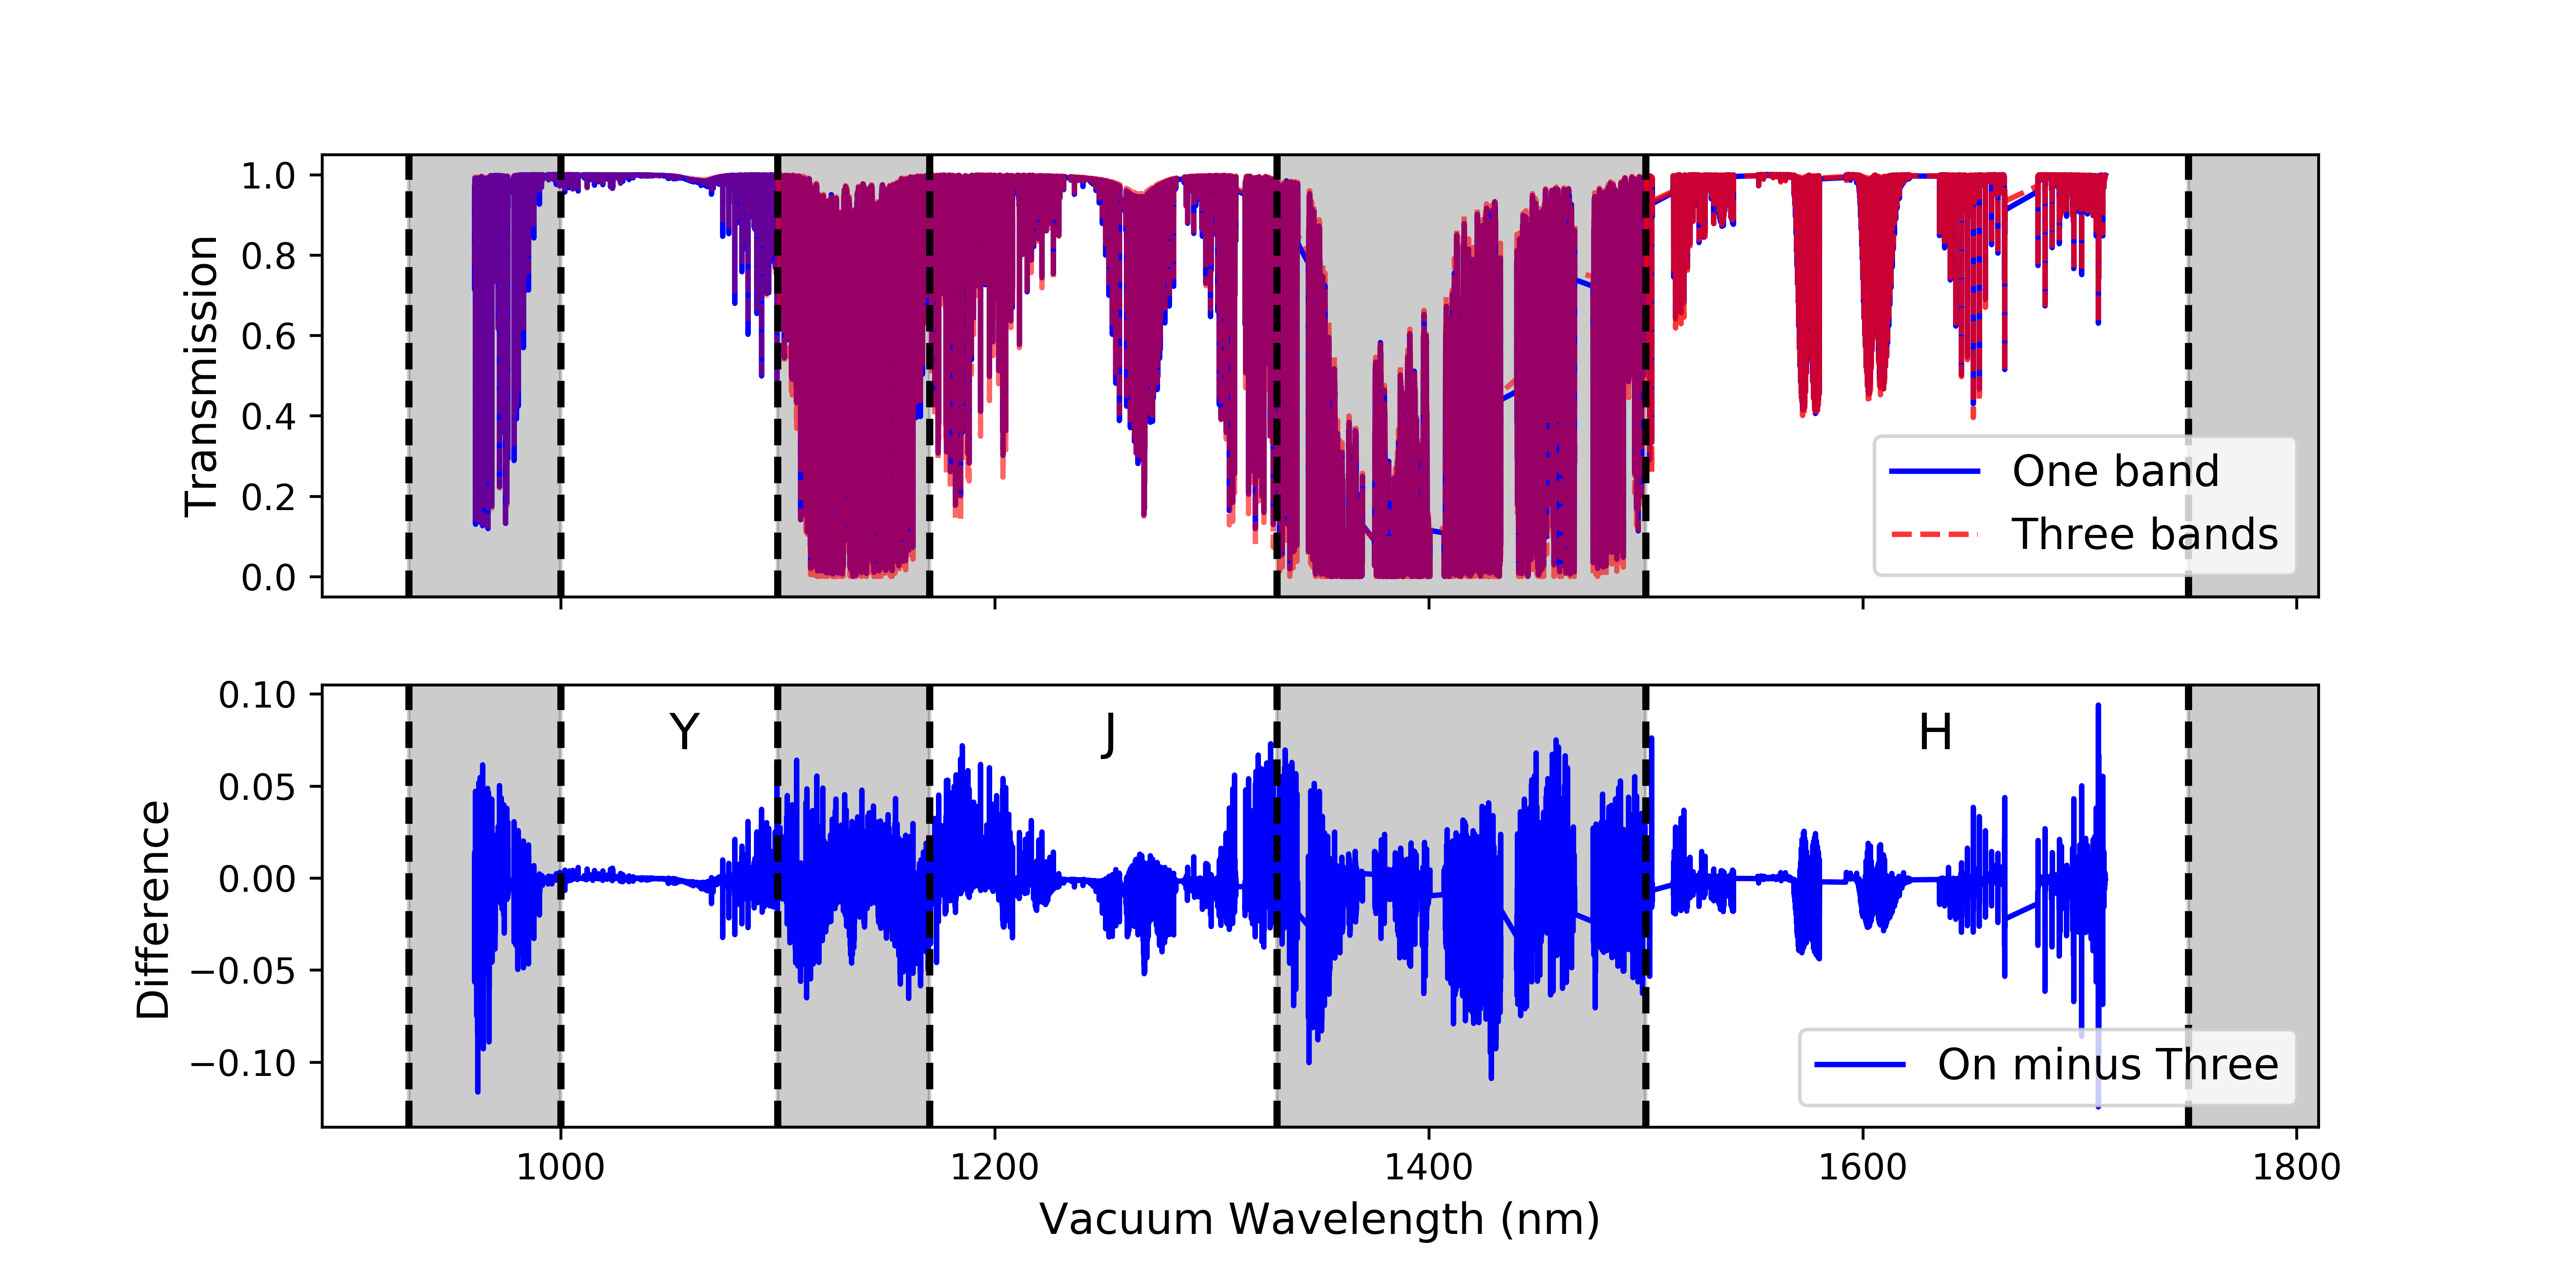
\includegraphics[width=0.9\linewidth]{figures/information-content/Carmenes/compare_telluric_corrections_shaded}
    \caption[]{Comparison of telluric models in pursuit of a better correction.
        Top: The two synthetic telluric spectra.
        The blue shows the result from {Molecfit} after treating the full spectrum as one, with a single spectral profile, while the shaded red telluric spectrum has been derived with three separate bands, fitted individually.
        Bottom: The difference in the telluric spectrum between the fit to the full spectrum, and the fit with the spectrum split into three.
        The regions of deep \ce{H2O} absorption lines which defined the \nir{} bands are shaded grey.
        The bounds of each band from \cref{tab:infrared_bands} are indicated with vertical black dashed lines.}
    \label{fig:compare_telluric_corrections}
\end{figure}


\begin{figure}
    \centering
    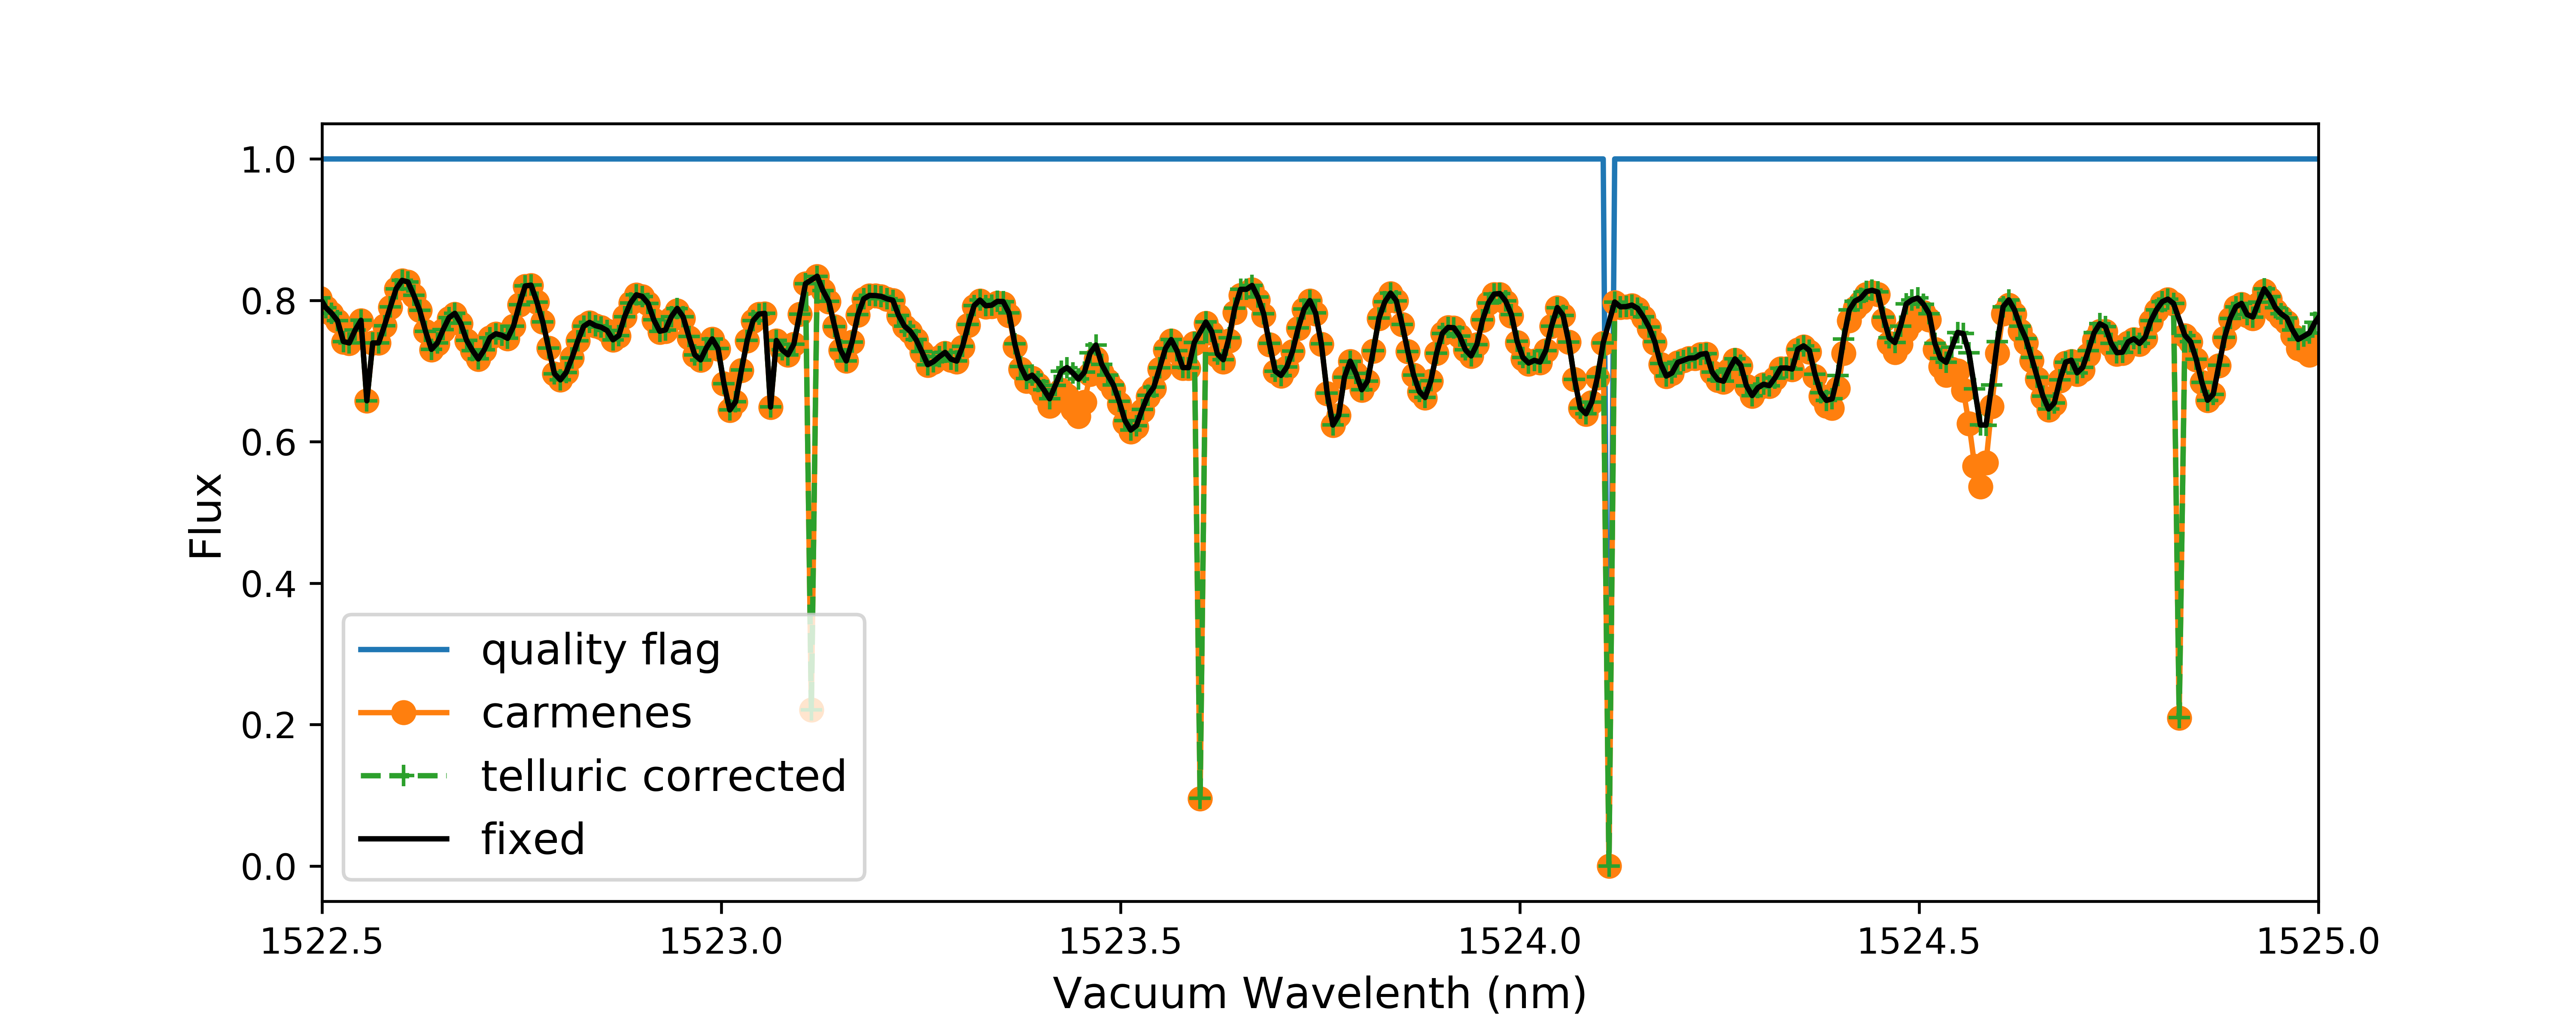
\includegraphics[width=0.9\linewidth]{figures/information-content/Carmenes/carmenes_spike_removal}
    \caption[Bad pixel removal in {CARMENES}.]{Removal of bad pixels from the {CARMENES} spectrum. The orange line with circles and green line with pluses are the original and telluric corrected spectra from {CARMENES}.
    The black solid line shows the spectrum after correction from bad pixels.
    The blue line shows the ``quality flag'' (0 or 1) output from the {Molecfit} software.}
    \label{fig:carmenes_spike_removal}
\end{figure}


\subsection{Impact of telluric correction}
\label{subsec:impact_telluric_correction}
Here the impact of the telluric correction on the spectral quality of the CARMENES spectrum is assessed.
This was done by calculating, Q, with the original telluric lines deeper than 2\% masked out, and with the telluric correction performed.
This was done for both fitting methods attempted with Molecfit and displayed in \cref{fig:band_qualityfromapplyingtelluriccorrection}.
The top panel shows the telluric corrected spectrum (orange) along with the telluric mask that was applied (blue).
The bottom panel shows the spectral quality for the three spectral bands \emph{Y}, \emph{J}, and \emph{H}.

\begin{figure}
    \centering
    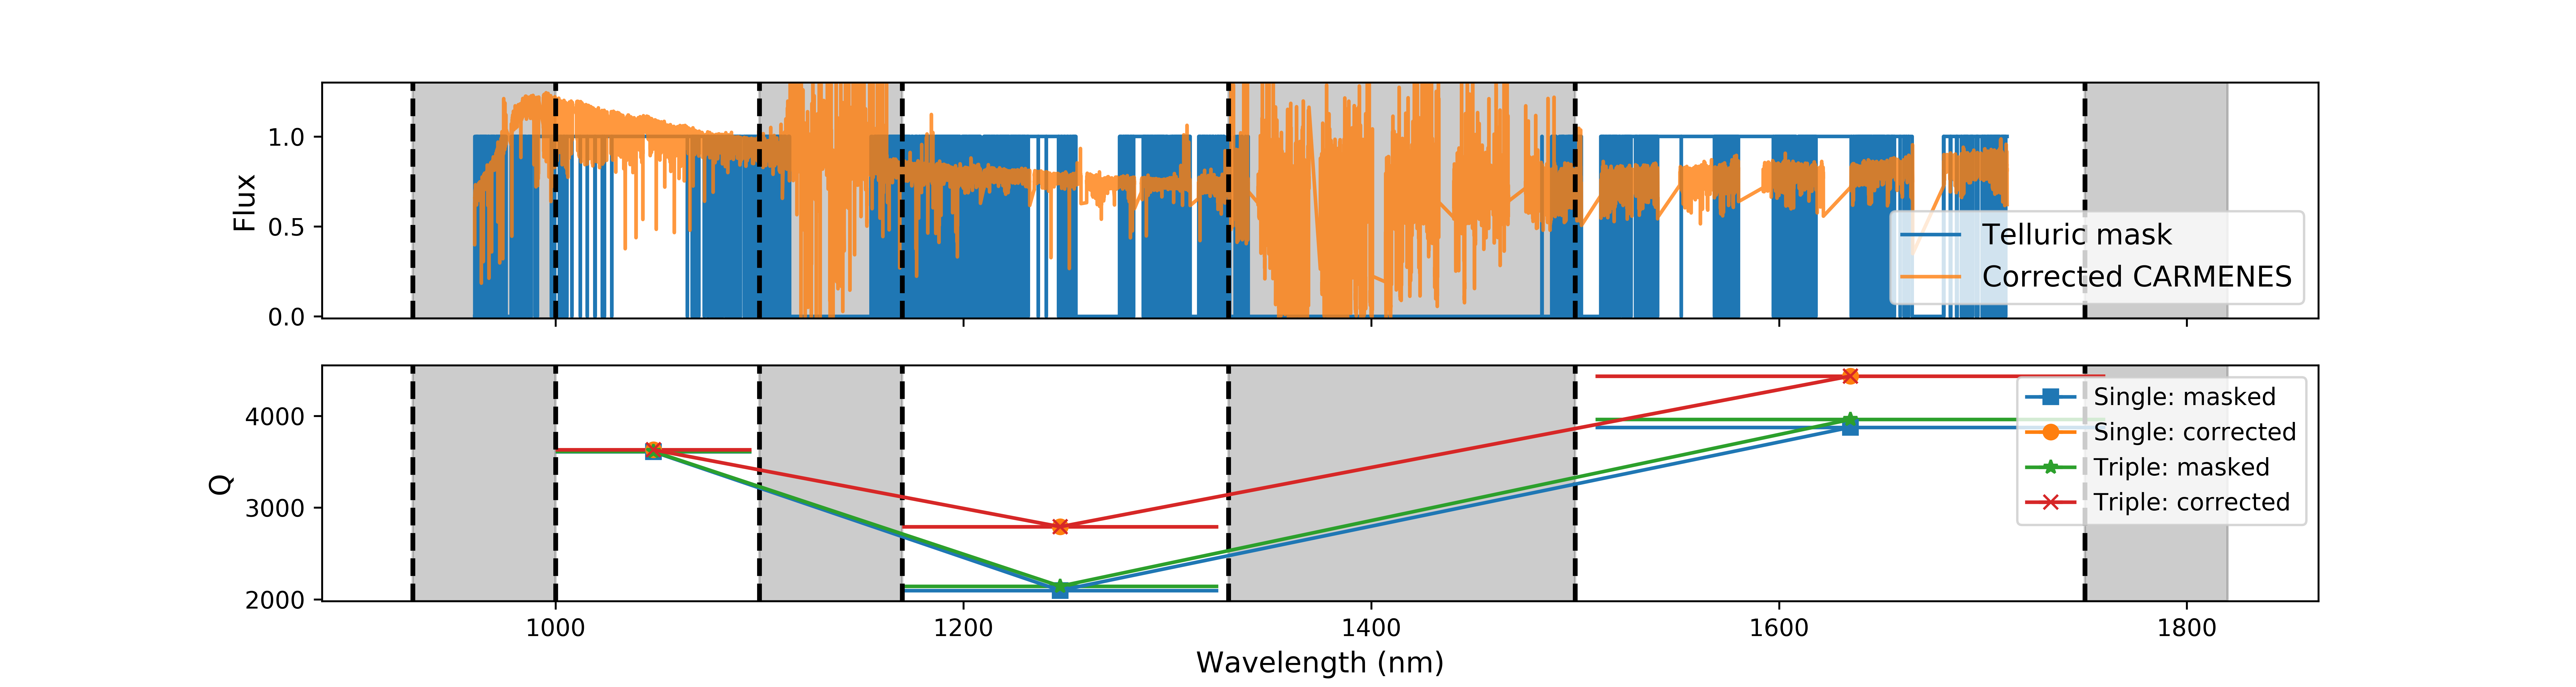
\includegraphics[width=0.8\linewidth]{figures/information-content/Carmenes/Band_quality_from_applying_telluric_correction}
    \caption[Barnard's star spectral quality.]{Measured spectral quality, Q, in the three \nir{} bands of Barnard's star to assess the gain from telluric correction. 
        Top: The telluric corrected CARMENES spectrum (orange) along with the binary mask for telluric lines >2\% depth (blue). 
        Bottom: The spectral quality in the three spectral bands, for different telluric treatment. `single' indicates the Molecfit results from the single fit to the spectrum, while `triple' indicates the fit to the three wavelength bands.
        `masked' indicates that telluric masking of the lines deeper than 2\% was performed and while `corrected' is just the telluric corrected spectrum.}
    \label{fig:band_qualityfromapplyingtelluriccorrection}
\end{figure}

\cref{fig:band_qualityfromapplyingtelluriccorrection} shows that there is a benefit (gain in quality) from telluric correction in the \emph{J} and \emph{H}-bands, where there are numerous telluric lines.
However, in the \emph{Y}-band where there is little telluric masking performed there is only a slight gain.
Performing telluric correction of the CARMENES spectra over telluric masking causes a gain the the spectral quality by 1\%, 30\%, 12\% in the \emph{Y}-band, \emph{J}, and \emph{H}-bands respectively.
As the spectral quality is related to the RV precision, this will lead to a 10-30\% improvement in the RV precision in the \emph{J}- and \emph{H}-bands
This indicated that it is worth performing telluric correction on the other seven {CARMENES} targets selected.
This also shows that the extra effort from three separate telluric fittings does not lead to a significant gain in quality.


\subsection{Barnard's star}
\label{sec:carmenes_barnards_star}
Currently only Barnard's star has had the telluric correction performed, and as such the analysis for this target is shown.
The spectral content of Barnard's star was extensively explored in~\citet{artigau_optical_2018} comparing the synthetic model to observations from {HARPS}, {ESPaDOns} and {CRIRES} in the range 380--2300\nm{}.
Agreement was found in the optical but the \nir{} bands had significant differences between the observations and models. 
The goal of this analysis is to check if the same results are obtainable in the {CARMENES} spectrum of Barnard's star.

\citet{artigau_optical_2018} tabulated several literature values for the stellar properties of Barnard's star and identified the closest matching {PHOENIX-ACES} model.
The synthetic model adopted for Barnard's star was \Teff=3200\K{}, \Logg{}=5.0, and \feh{}=-0.5, and we adopt the same model here.
This is tabulated in with other parameters from~\citet{artigau_optical_2018} in \cref{tab:barnards_star_params}.

\begin{table}
    \centering
    \caption[Properties of Barnard's star.]{Properties of Barnard's star from~\citet{artigau_optical_2018}. \Teff{}, \feh{} and \Logg{} values are only the adopted (closest) model parameters.}
    \begin{tabular}{lc}
        \toprule
        Parameter & Value \\
        \midrule
        SpType & M4\,Ve \\
        Rotation Period & \(\sim\)130 days \\
        \Vsini{} & \(\le 80\) \si{\metre\per\second} \\
        \Teff{} & 3200 \K{} \\
        \Logg{} & 5.0 \\
        \feh{} & -0.5 \\
        \bottomrule{}
    \end{tabular}\label{tab:barnards_star_params}
\end{table}

A series of spectra are shown in \cref{fig:carmenes_correction}.
The uncorrected {CARMENES} spectrum of Barnard's Star is shown in the first panel.
The second panel shows telluric model from Molecfit, while the third panel shows the telluric corrected spectrum.
In the telluric corrected spectrum there are several deep spikes which are bad pixels.
Most of these are corrected for in the fourth panel, although it appears there may be a few still present in the spectrum.
The fifth panel contains the synthetic PHOENIX-ACES spectrum of Barnard's star, used to compare the spectral quality.
The model has been convolved by an instrumental profile with R=80\,400, but not rotationally broadened since the \Vsini{} is low. The flux units of the spectra are arbitrary, and the synthetic model has been converted into photon counts.

\begin{figure}
    \centering
    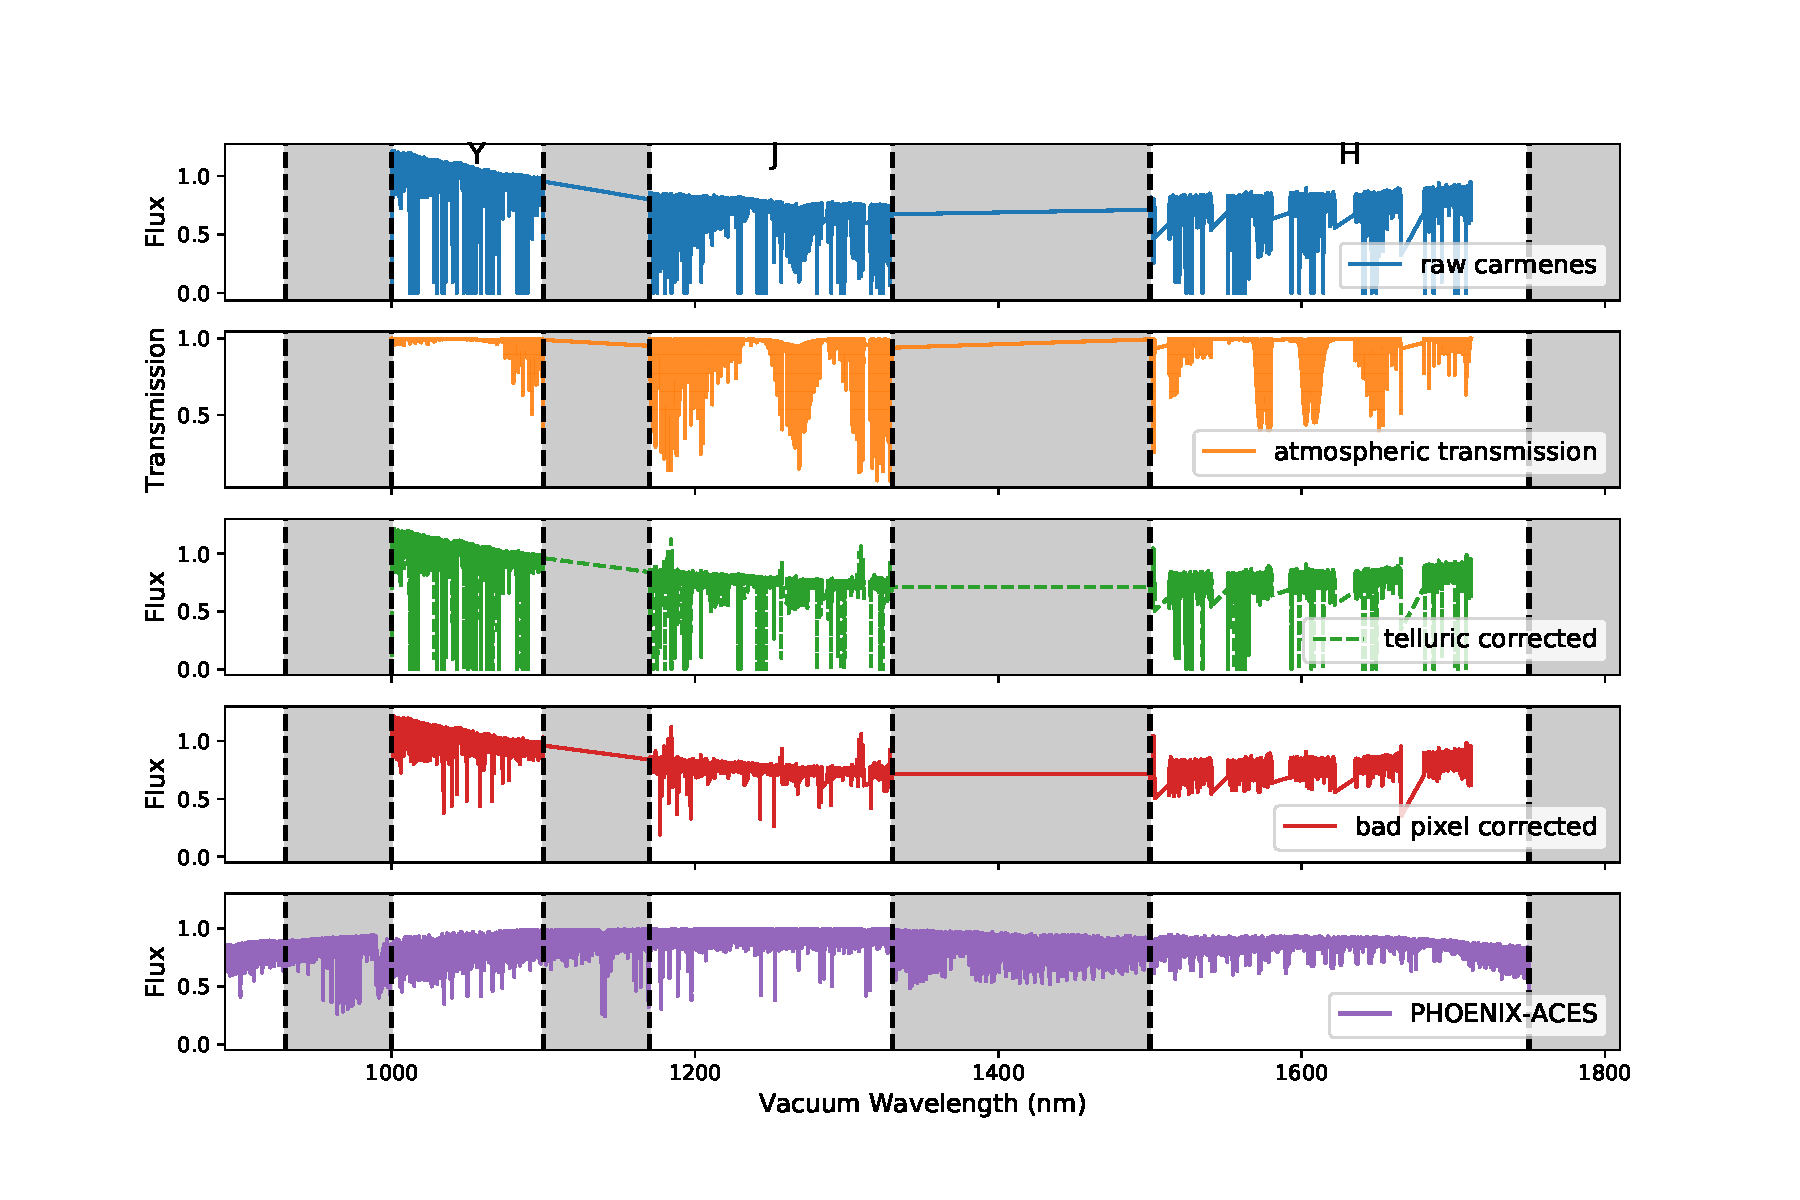
\includegraphics[width=0.8\linewidth]{figures/information-content/Carmenes/bp_carmenes_masked_model_broadened}
    \caption[Telluic correction of the {CARMENES} \nir{} spectrum.]{Telluic correction of the {CARMENES} \nir{} spectrum.
        First: Uncorrected spectrum of Barnard's Star between 960--1710\nm{} from {CARMENES}.
        Second: The synthetic telluric transmission spectrum fitted with {Molecfit}.
        Third: Telluric corrected spectrum by division of the telluric spectrum.
        The regions of deep \ce{H2O} absorption lines which defined the \nir{} bands are shaded grey.
        Fourth: The telluric corrected spectra after the bad pixels are removed.
        Fifth: Synthetic PHOENIX-ACES model for Barnard's star, convolved to R=80\,400.
        The bounds of each band from \cref{tab:infrared_bands} are indicated with vertical black dashed lines.
        The flux units of the spectra are arbitrary}
    \label{fig:carmenes_correction}
\end{figure}


To compare the model to the observation it is interpolated to the pixel positions of the {CARMENES} spectrum.
The spectral quality is calculated for both on small wavelength bins with a width 0.2\% the central wavelength similar to~\citet{artigau_optical_2018}.
The top panel of \cref{fig:qualitycomparisiontomodel} shows the results of the comparison, with the spectral quality in 0.2\%\,\(\lambda\) width bins for the observation (orange squares) and the model (blue stars) in the top panel.
The ratio between the spectral quality of the observation and the model is given in the bottom panel.
It shows that in this instance the \emph{Y}- and \emph{J}-bands have a similar spectral quality, while there is a large difference in the \emph{H}-band with the CARMENES observation having a spectral quality 3--4\(\times\) greater than the model.

\begin{figure}
    \centering
    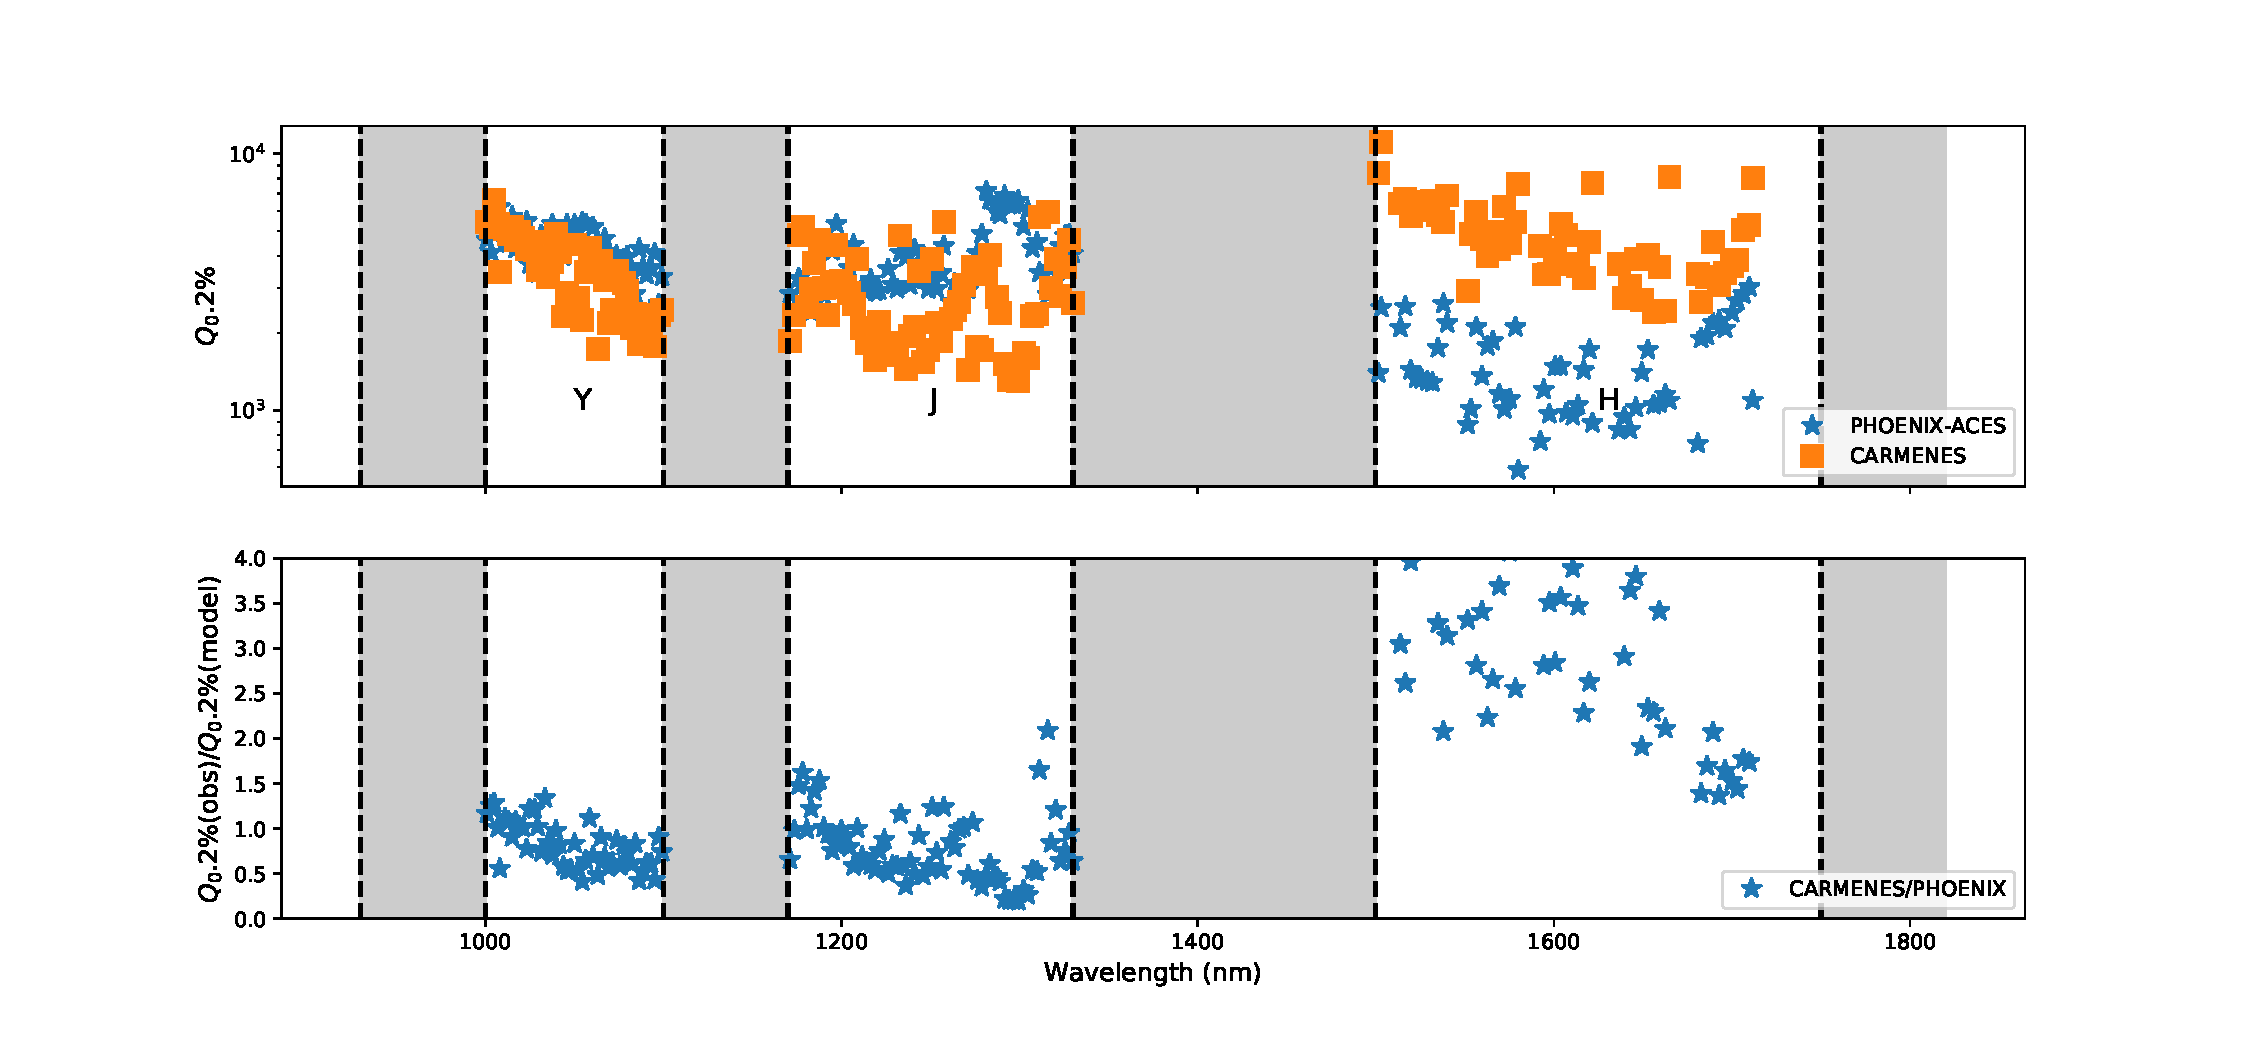
\includegraphics[width=0.8\linewidth]{figures/information-content/Carmenes/quality_comparision_to_model}
    \caption[Barnard's star spectral quality compared to CARMENES.]{Measured RV content of Barnard's star over the near-infrared domain, from CARMENES.
    Top: The spectral quality in 0.2\%\,\(\lambda\) width bins for CARMENES (orange squares) and the model (blue stars).
    Bottom: The ratio of spectral quality observed/model.}
    \label{fig:qualitycomparisiontomodel}
\end{figure}

For comparison the corresponding image from~\citet{artigau_optical_2018} is provided in \cref{fig:allw2}.
It shows a lower computed spectral quality (50\%) in the \emph{Y}- and \emph{J}-bands compared to the model of Barnard's star.
However in this work the model and observation have a similar spectral quality in these bands, although the ratio does drop to 50\% towards the red end of the \emph{J}-band.
In the \emph{H}-band of both works the observed quality is higher then the model, however the CARMENES spectral quality is 3\(\times\) higher, instead of only 1.5\(\times\) in~\citet{artigau_optical_2018}.
This is a significant difference.

\citet{artigau_optical_2018} only apply telluric masking in their analysis, whereas here the telluric corrected spectra were used.
This could be part of the reason for the largely improved results in the \emph{H}.
As shown in \cref{subsec:impact_telluric_correction} the telluric correction can improve the quality by 12--30\%.
However, this does not fully explain the increase by a factor of 2.
This requires further investigation.


\begin{figure}
    \centering
    \begin{tabular}{c}
    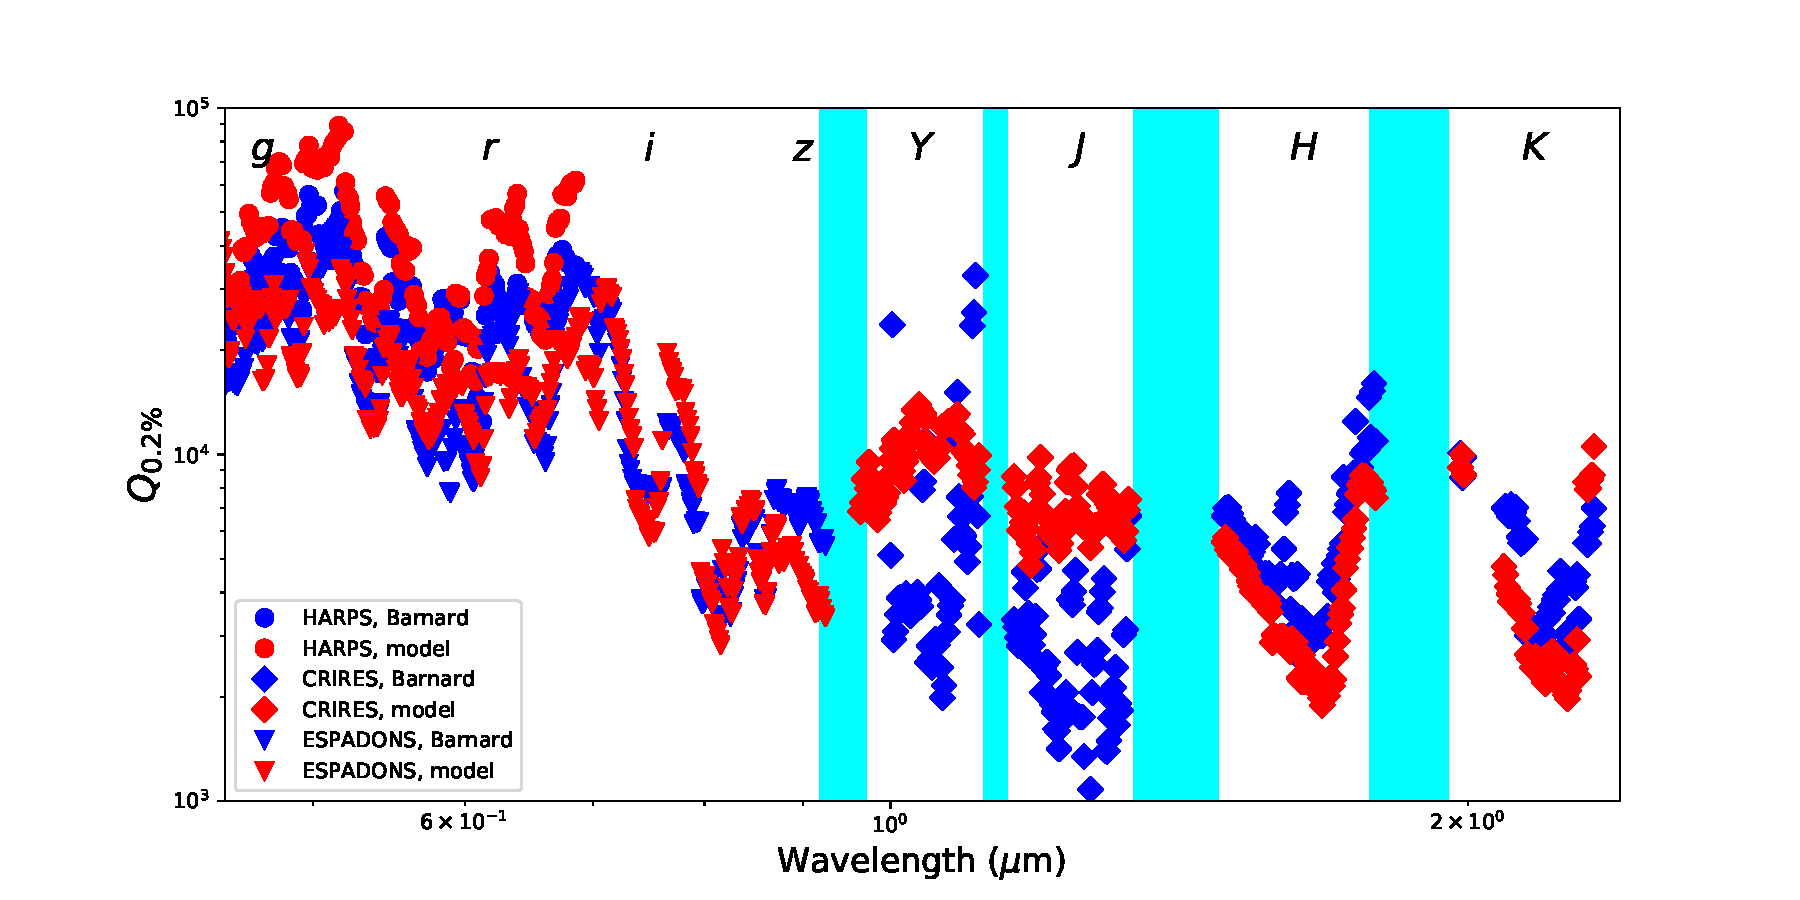
\includegraphics[width=0.8\linewidth]{figures/information-content/artigau2018_figures/all_w}\\
    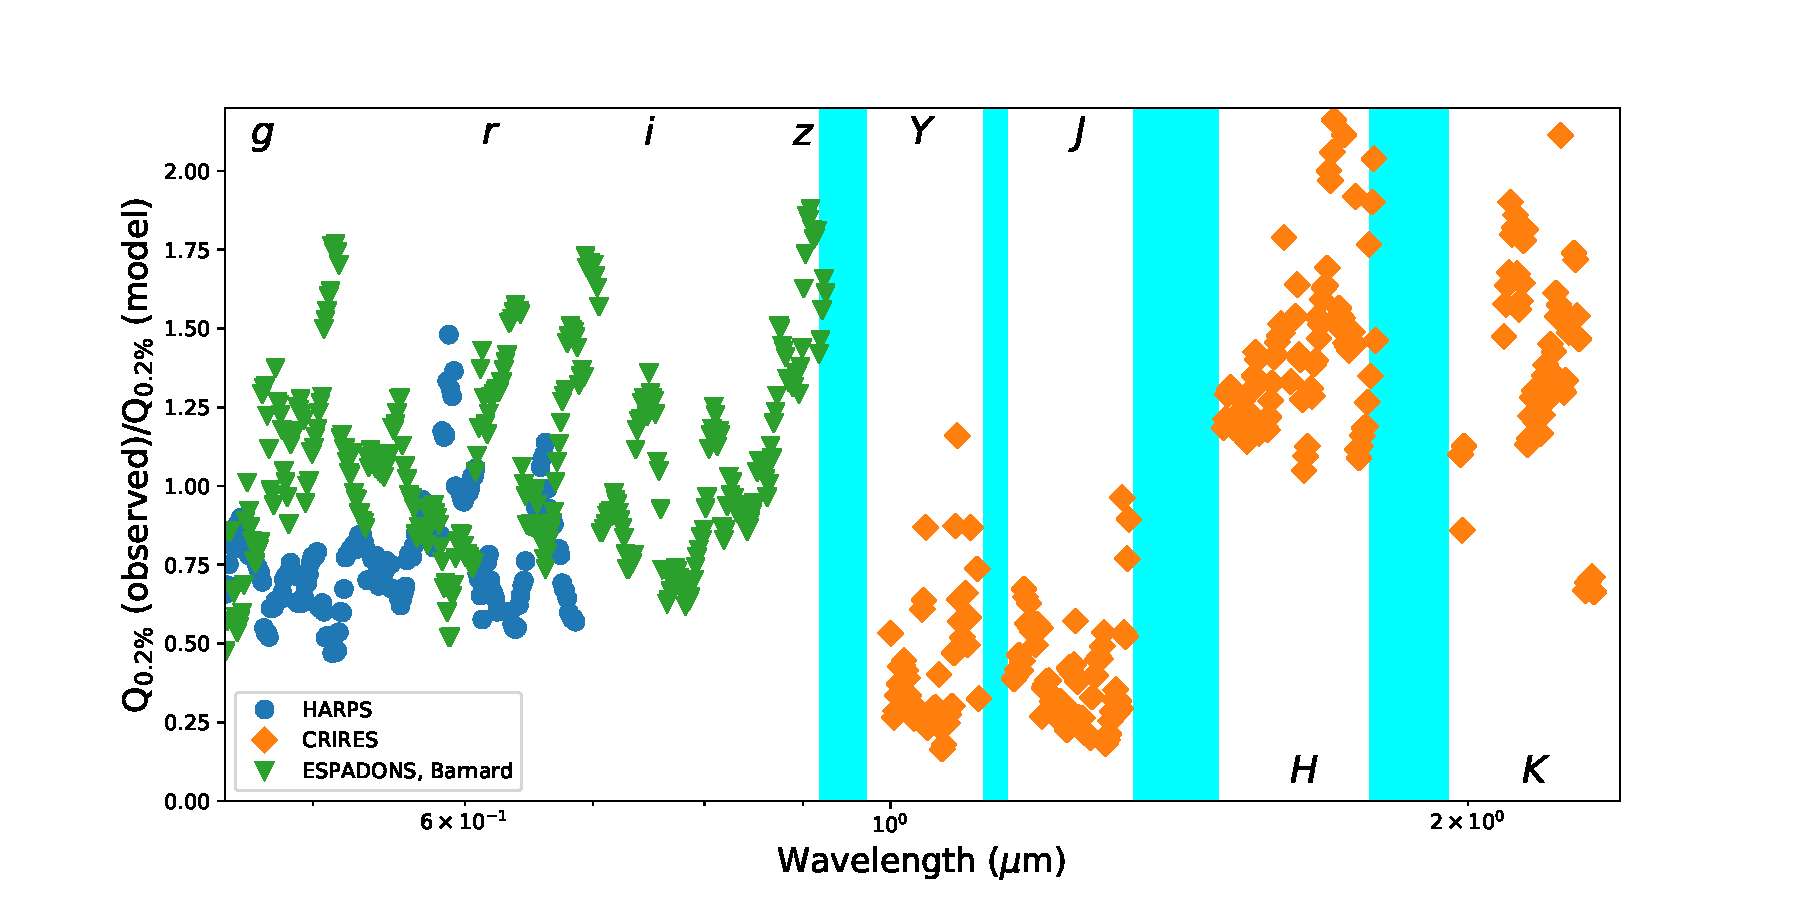
\includegraphics[width=0.8\linewidth]{figures/information-content/artigau2018_figures/all_w2}
    \end{tabular}
    \caption[Measured RV content of Barnard's star over the optical and near-infrared domain.]{Measured RV content of Barnard's star over the optical and near-infrared domain. Overall measured (blue) and model (red) RV density are well matched blueward of $\sim1\mu$m. The agreement is poorer in the near-infrared domain with an over-prediction of RV content in $Y$ and \emph{J} bands and an under-prediction in \emph{H} and \emph{K}.
    Bottom: Ratio of observed to model $Q_{0.2\%}$ values. Areas unusable for RV measurements because of strong telluric absorption are filled in light blue. Reproduced from~\citet{artigau_optical_2018}.}
    \label{fig:allw2}
\end{figure}


%This work specifically added an extra feature to \eniric{} in the ability to calculate the precision on shorter wavelength scales rather than the full band. This is inspired and driven by the wavelength bins with a width \(2\%\times\lambda^\prime\), centred at \(\lambda^\prime\) as done in~\citep{artigau_optical_2018}.
%This allows for a finer resolution of the spectral quality throughout the band rather than just the full band
%precision as done in~\citet{figueira_radial_2016} and \cref{fig:band_qualityfromapplyingtelluriccorrection}.
%Analysis of the precision on smaller wavelength scales is also performed in other works~\citep[e.g.][]{bouchy_fundamental_2001, reiners_carmenes_2018}.


\subsubsection{Future tasks}
\label{subsubsec:future_tasksaims}
These results are still preliminary analyses, and a few things can be improved.
For instance the observed and model spectra have not yet been Doppler shifted to the same frame.
A Doppler shift of a few \nm{} is unlikely to affect the results shown in \cref{fig:qualitycomparisiontomodel} significantly.
There are also a few bad pixels that are still present in the observation that should be properly removed.

Adding the analysis of several CARMENES spectra across the M-dwarf range would be an important addition to this work to see if these results are consistent for all spectra, or if they are dependant on the stellar parameters.

